\section{Resultados}
\label{sec:resultados}

\graphicspath{{img/}{../img/}{../../img/}}

\pgfplotstableread[col sep=comma]{../../results/wing_degree_sweep.csv}\wingdegreesweep
\pgfplotstableread[col sep=comma]{../../results/wing_full_fit_metrics.csv}\wingfullfit
\pgfplotstableread[col sep=comma]{../../results/benchmark_scaling.csv}\benchmarkscaling
\pgfplotstableread[col sep=comma]{../../results/benchmark_high_load.csv}\benchmarkhigh
\pgfplotstableread[col sep=comma]{../../results/regkit_usage_rmse.csv}\regkitusagermse

\pgfplotstablegetelem{2}{test_r2}\of\wingdegreesweep
\edef\wingDegreeFourRtwo{\pgfplotsretval}
\pgfplotstablegetelem{4}{test_r2}\of\wingdegreesweep
\edef\wingDegreeSixRtwo{\pgfplotsretval}
\pgfplotstablegetelem{5}{test_r2}\of\wingdegreesweep
\edef\wingDegreeSevenRtwo{\pgfplotsretval}

\pgfplotstablegetelem{0}{rmse}\of\wingfullfit
\edef\wingFullRmse{\pgfplotsretval}
\pgfplotstablegetelem{0}{r2}\of\wingfullfit
\edef\wingFullRtwo{\pgfplotsretval}

\pgfplotstablegetelem{3}{Mean time [s]}\of\benchmarkscaling
\edef\benchNaiveTime{\pgfplotsretval}
\pgfplotstablegetelem{3}{Peak memory [MB]}\of\benchmarkscaling
\edef\benchNaiveMem{\pgfplotsretval}
\pgfplotstablegetelem{4}{Mean time [s]}\of\benchmarkscaling
\edef\benchOptTime{\pgfplotsretval}
\pgfplotstablegetelem{4}{Peak memory [MB]}\of\benchmarkscaling
\edef\benchOptMem{\pgfplotsretval}
\pgfplotstablegetelem{5}{Mean time [s]}\of\benchmarkscaling
\edef\benchOocTime{\pgfplotsretval}
\pgfplotstablegetelem{5}{Peak memory [MB]}\of\benchmarkscaling
\edef\benchOocMem{\pgfplotsretval}

\pgfplotstablegetelem{0}{Mean time [s]}\of\benchmarkhigh
\edef\benchHighOptTime{\pgfplotsretval}
\pgfplotstablegetelem{0}{Peak memory [MB]}\of\benchmarkhigh
\edef\benchHighOptMem{\pgfplotsretval}
\pgfplotstablegetelem{1}{Mean time [s]}\of\benchmarkhigh
\edef\benchHighOocTime{\pgfplotsretval}
\pgfplotstablegetelem{1}{Peak memory [MB]}\of\benchmarkhigh
\edef\benchHighOocMem{\pgfplotsretval}

\pgfplotstablegetelem{0}{rmse}\of\regkitusagermse
\edef\explorationNaiveOneRmse{\pgfplotsretval}
\pgfplotstablegetelem{9}{rmse}\of\regkitusagermse
\edef\explorationOptFiveRmse{\pgfplotsretval}
\pgfplotstablegetelem{11}{rmse}\of\regkitusagermse
\edef\explorationOptSevenRmse{\pgfplotsretval}

\pgfplotstablegetelem{25}{rmse}\of\regkitusagermse
\edef\targetDegreeOneRmse{\pgfplotsretval}
\pgfplotstablegetelem{27}{rmse}\of\regkitusagermse
\edef\targetDegreeThreeRmse{\pgfplotsretval}
\pgfplotstablegetelem{29}{rmse}\of\regkitusagermse
\edef\targetDegreeFiveRmse{\pgfplotsretval}
\pgfplotstablegetelem{31}{rmse}\of\regkitusagermse
\edef\targetDegreeSevenRmse{\pgfplotsretval}

\edef\wingDegreeFourRtwoPercent{\fpeval{100*\wingDegreeFourRtwo}}
\edef\wingDegreeSixRtwoPercent{\fpeval{100*\wingDegreeSixRtwo}}
\edef\wingDegreeSevenRtwoPercent{\fpeval{100*\wingDegreeSevenRtwo}}
\edef\wingFullRtwoPercent{\fpeval{100*\wingFullRtwo}}

\edef\benchSpeedup{\fpeval{\benchNaiveTime/\benchOptTime}}
\edef\benchMemPercent{\fpeval{100*(\benchOptMem/\benchNaiveMem)}}
\edef\benchOocTimeVar{\fpeval{100*abs((\benchOocTime-\benchOptTime)/\benchOptTime)}}
\edef\benchOocMemVar{\fpeval{100*abs((\benchOocMem-\benchOptMem)/\benchOptMem)}}
\edef\benchHighTimeDrop{\fpeval{100*(1-\benchHighOocTime/\benchHighOptTime)}}

\subsection{Problema 1: hélices exploratórias}

A Figura~\ref{fig:exploratorio} apresenta a projeção PCA do conjunto helicoidal
gerado por \texttt{gen\_exploration\_dataset}. Com $n=3$, $m=2$ e
$N=200$ amostras, o ruído gaussiano de desvio padrão $0{,}01$ não impede que o
modelo otimizado recupere a geometria latente: os pontos originais e as
predições praticamente se sobrepõem para graus acima de cinco. O RMSE cai de
\num{\explorationNaiveOneRmse} (grau~1) para \num{\explorationOptFiveRmse}
(grau~5), confirmando que a montagem vetorizada preserva a mesma dinâmica do
protótipo simbólico descrito na Seção~\ref{sec:metodologia}.

\begin{figure}[H]
    \centering
    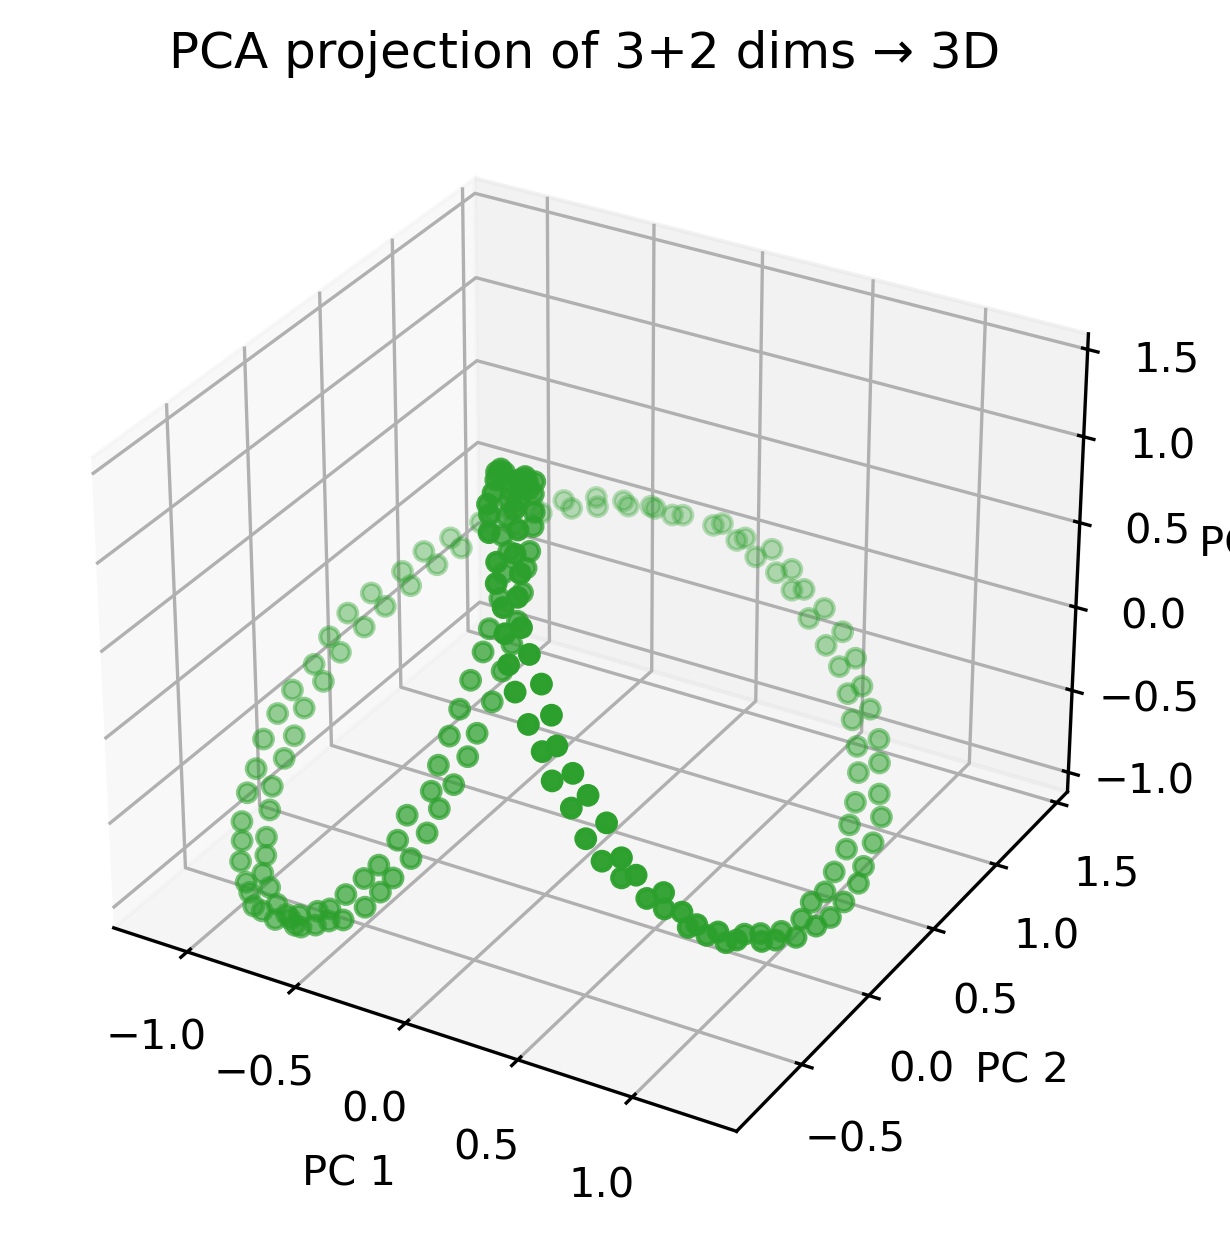
\includegraphics[width=0.75\linewidth]{usage_dataset.png}
    \caption{Projeção PCA do conjunto exploratório com $N=200$ amostras.}
    \label{fig:exploratorio}
\end{figure}

O impacto do grau polinomial aparece na Figura~\ref{fig:exploratorio-sweep}.
O ganho geométrico é evidente ao comparar os graus 1 e~6: o primeiro apenas
captura o esqueleto helicoidal, enquanto o segundo já reproduz os enrolamentos
laterais da trajetória. O gráfico de erro indica retornos rapidamente
decrescentes após o grau~7, quando o RMSE atinge
\num{\explorationOptSevenRmse}. A queda quase linear no painel logarítmico
evidencia que termos de ordem superior refinam as regiões de maior curvatura sem
degradar o condicionamento, efeito habilitado pelas rotinas de regularização
automática discutidas na Seção~\ref{sec:metodologia}.

\begin{figure}[H]
    \centering
    \begin{minipage}{0.48\linewidth}
        \centering
        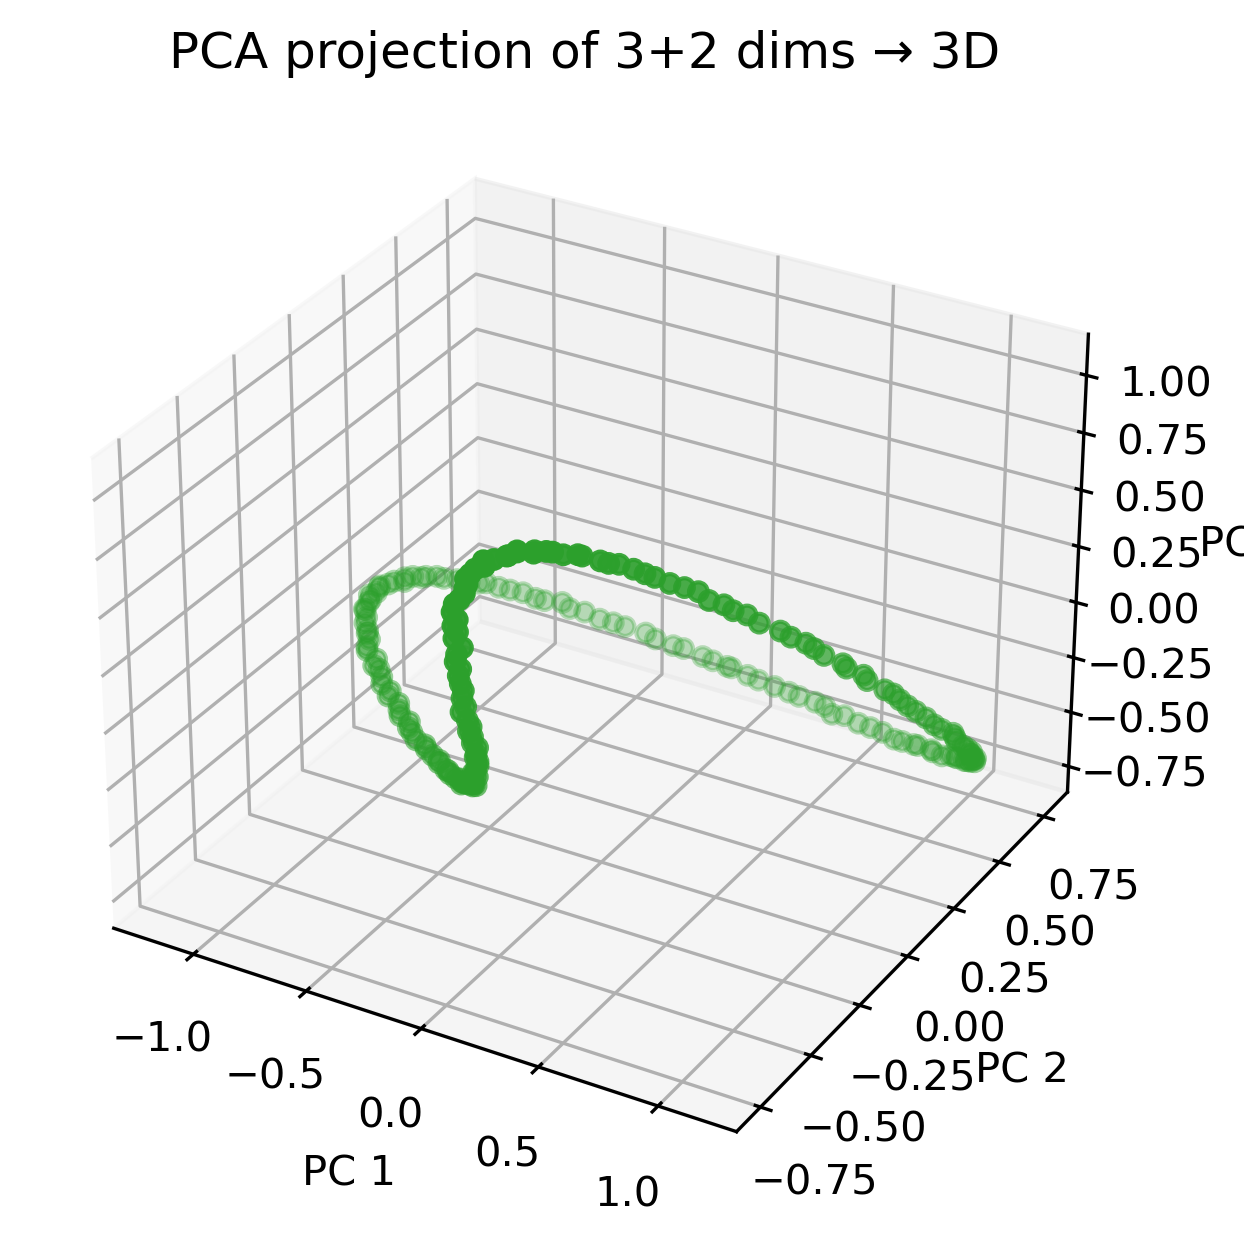
\includegraphics[width=\linewidth]{usage_naive_degree_1.png}\\[0.5em]
        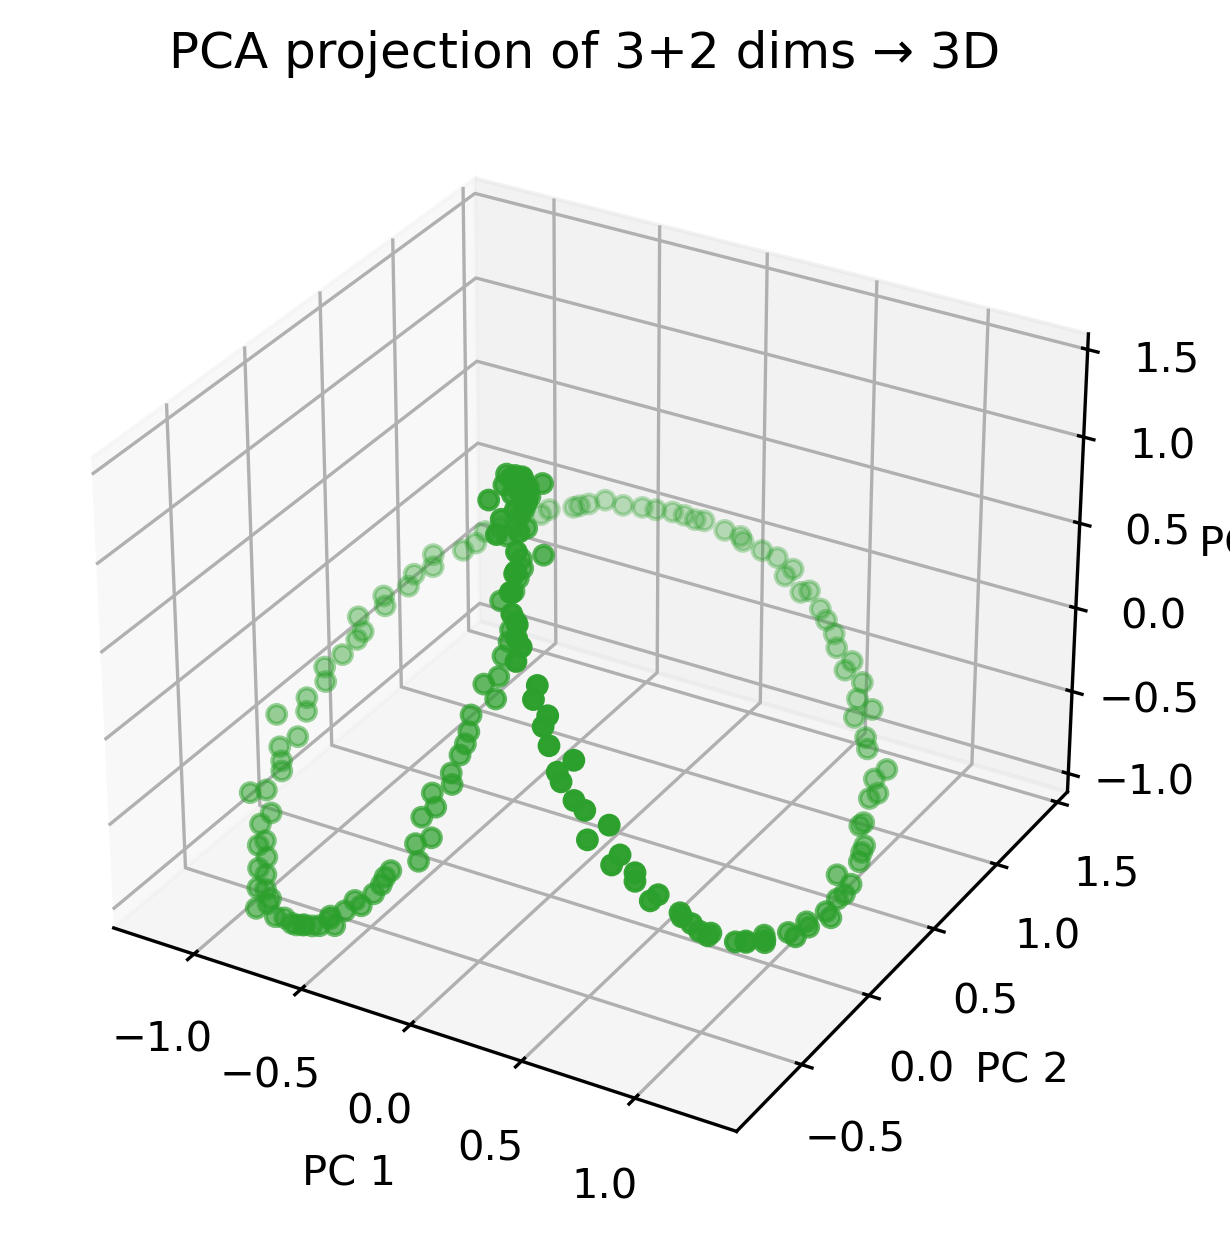
\includegraphics[width=\linewidth]{usage_naive_degree_6.png}
    \end{minipage}\hfill
    \begin{minipage}{0.48\linewidth}
        \centering
        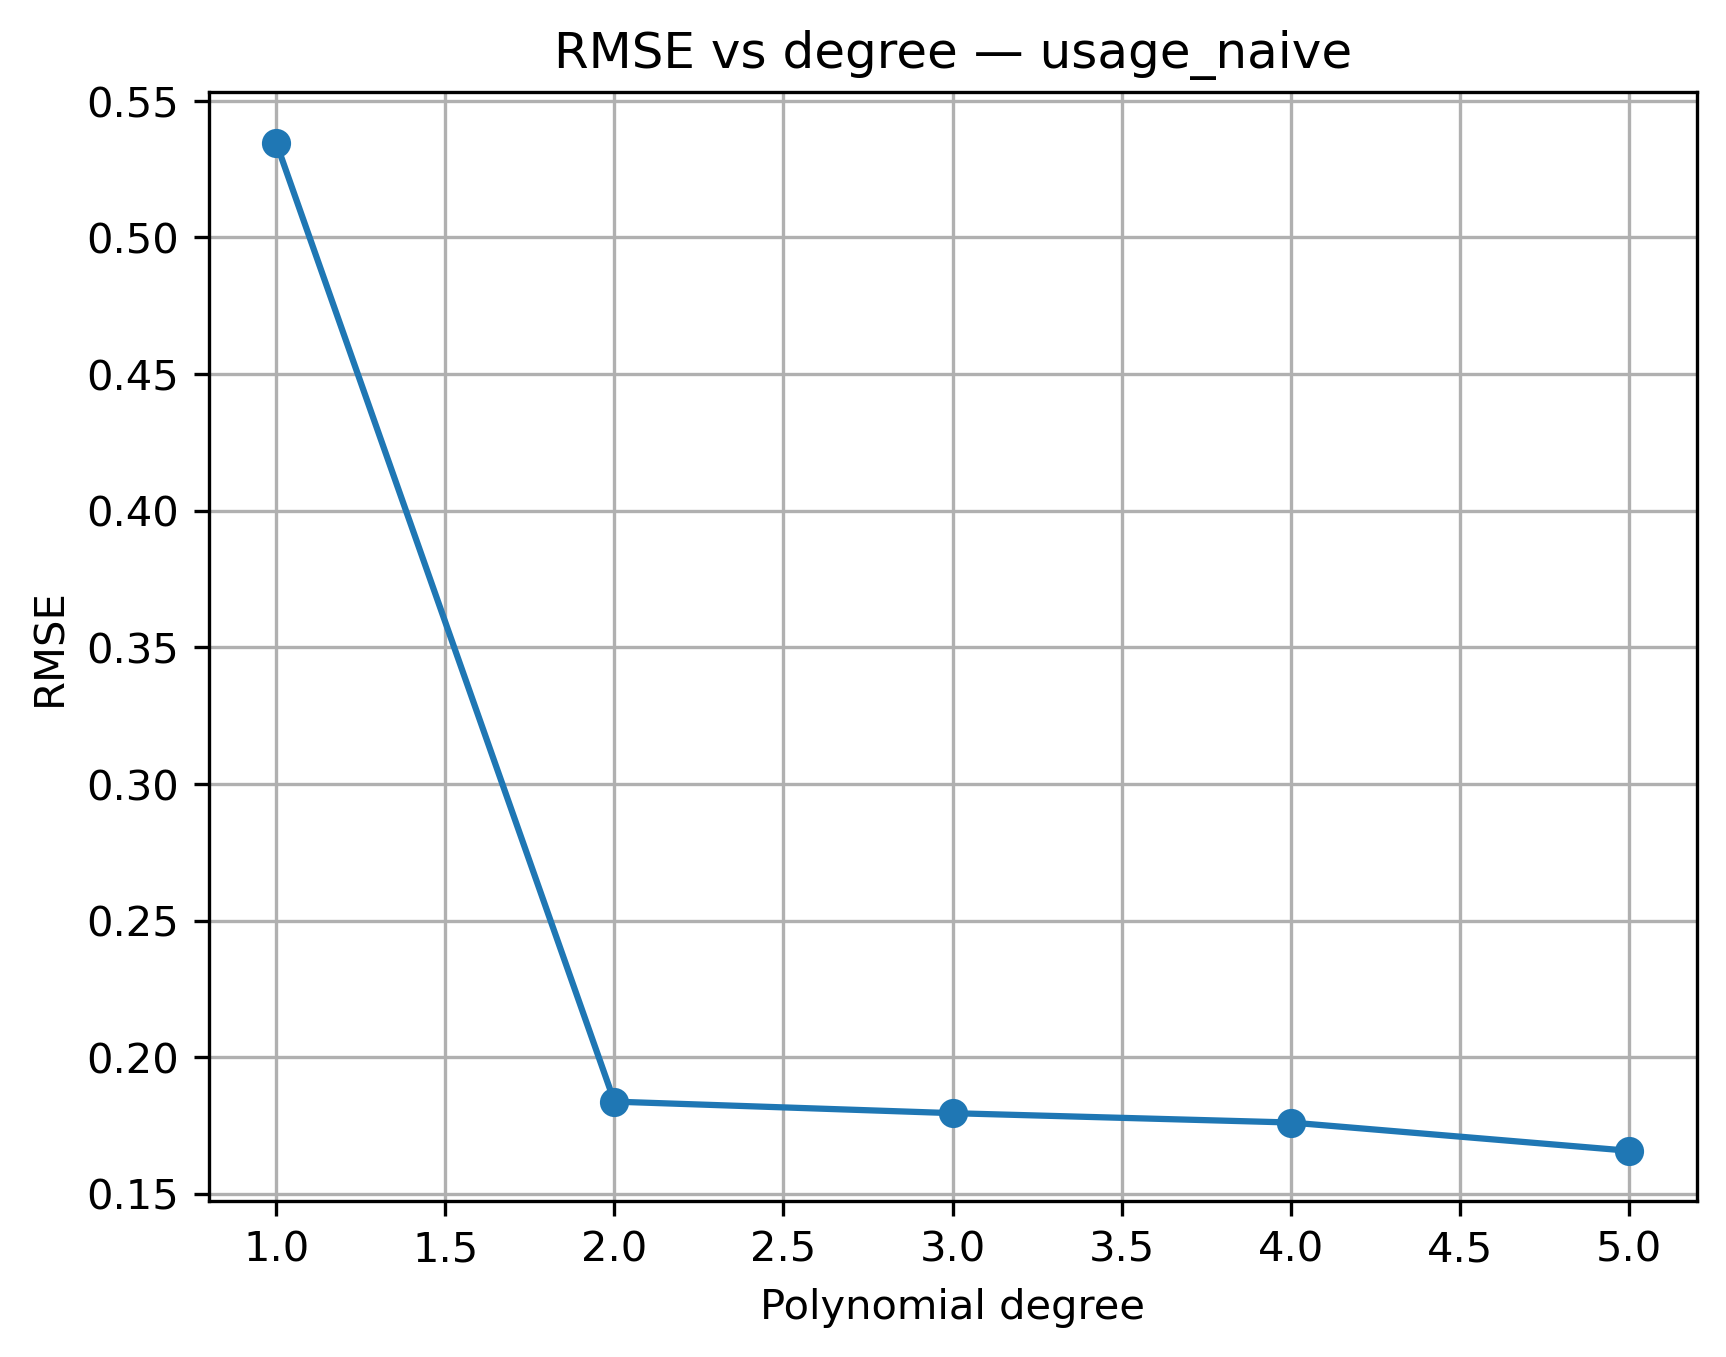
\includegraphics[width=\linewidth]{usage_naive_rmse.png}\\[0.5em]
        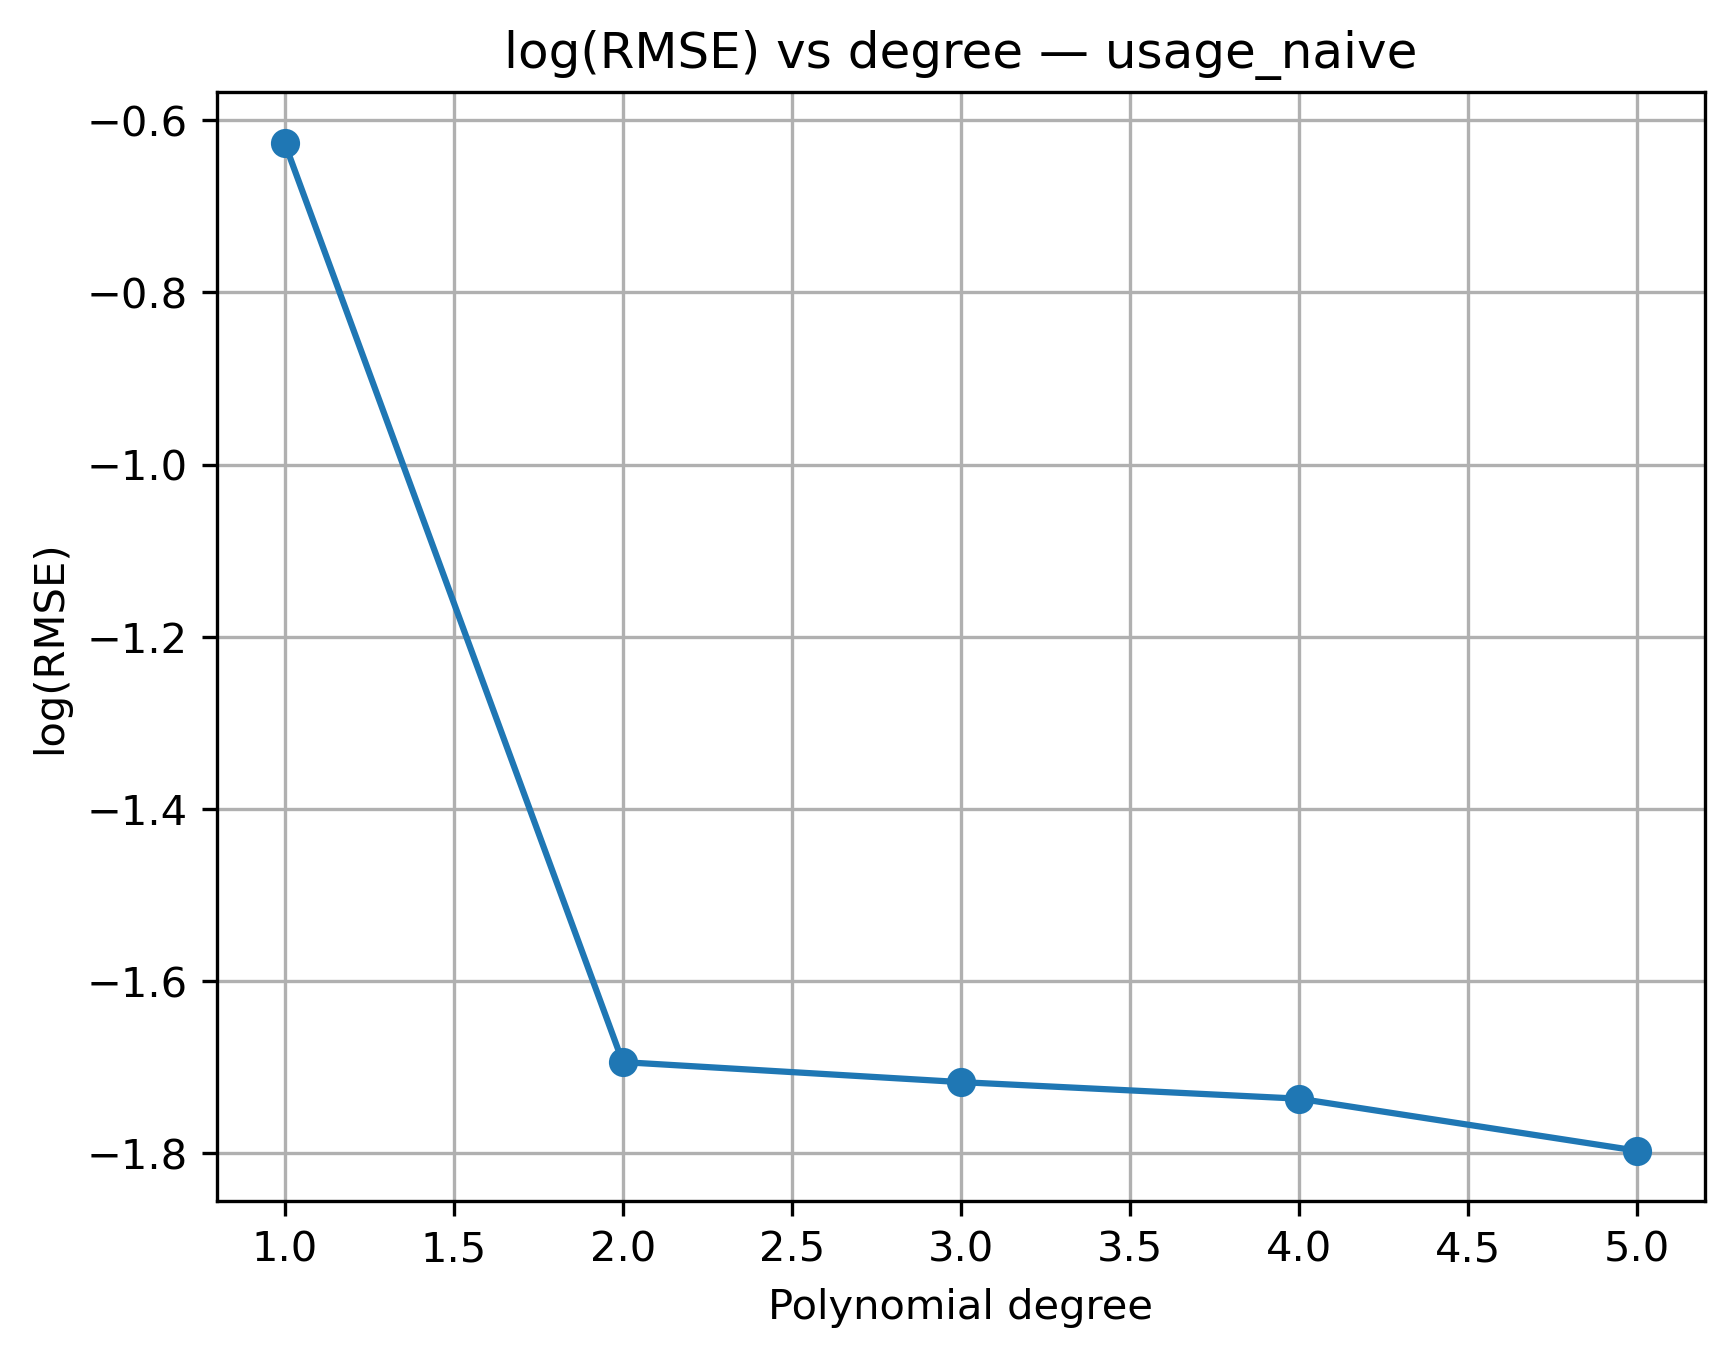
\includegraphics[width=\linewidth]{usage_naive_rmse_log.png}
    \end{minipage}
    \caption{Impacto do grau polinomial. Na esquerda há projeções para os polinômios de grau 1 e 6 e, na direita há o RMSE absoluto e
    logarítmico.}
    \label{fig:exploratorio-sweep}
\end{figure}

\subsection{Problema 2: protótipo 4$\times$4}

O protótipo~4$\times$4 reproduz o conjunto distribuído com o projeto e
combina quatro entradas com quatro saídas correlacionadas. A projeção PCA da
Figura~\ref{fig:target-dataset} mostra que o modelo otimizado acompanha os dois
regimes independentes do problema: as curvas parametrizadas por $t$ e a faixa de
valores controlada por $q$. A trajetória do RMSE cai de
\num{\targetDegreeOneRmse} (grau~1) para
\num{\targetDegreeThreeRmse} (grau~3),
\num{\targetDegreeFiveRmse} (grau~5) e alcança
\num{\targetDegreeSevenRmse} no grau~7, como resume a
Figura~\ref{fig:target-metrics}. O comportamento quase polinomial no painel
logarítmico revela que os termos de grau ímpar absorvem as principais
interações entre os parâmetros, deixando resíduos próximos à precisão numérica.

\begin{figure}[H]
    \centering
    \begin{minipage}{0.48\linewidth}
        \centering
        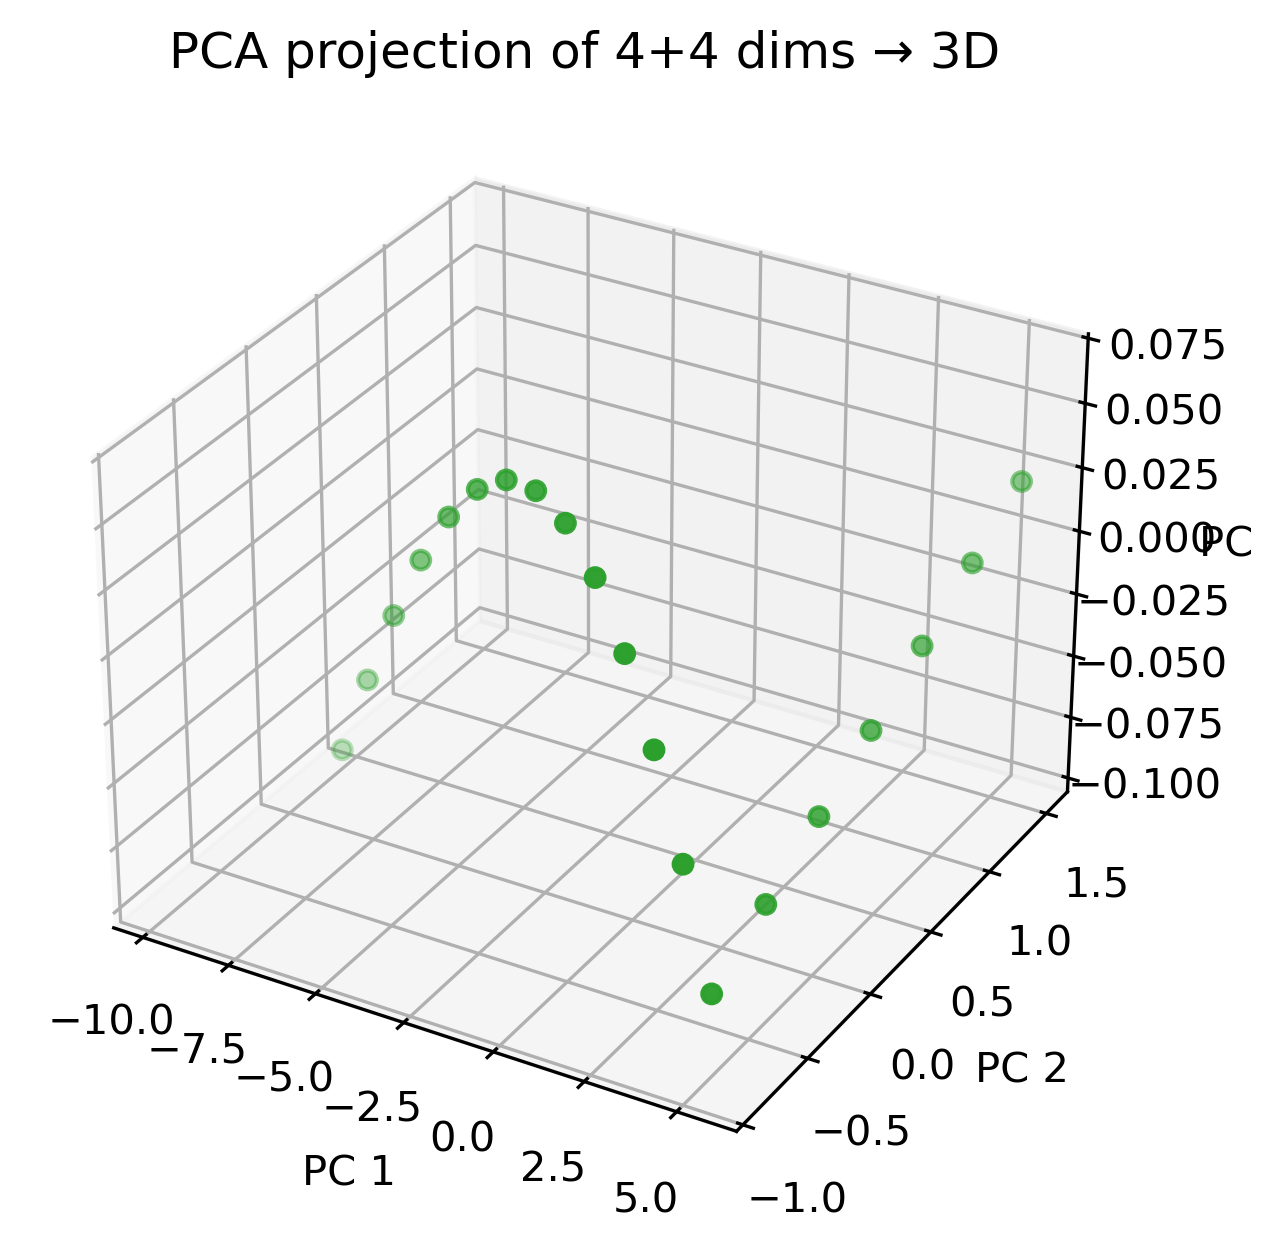
\includegraphics[width=\linewidth]{usage_target_dataset.png}\\[0.5em]
        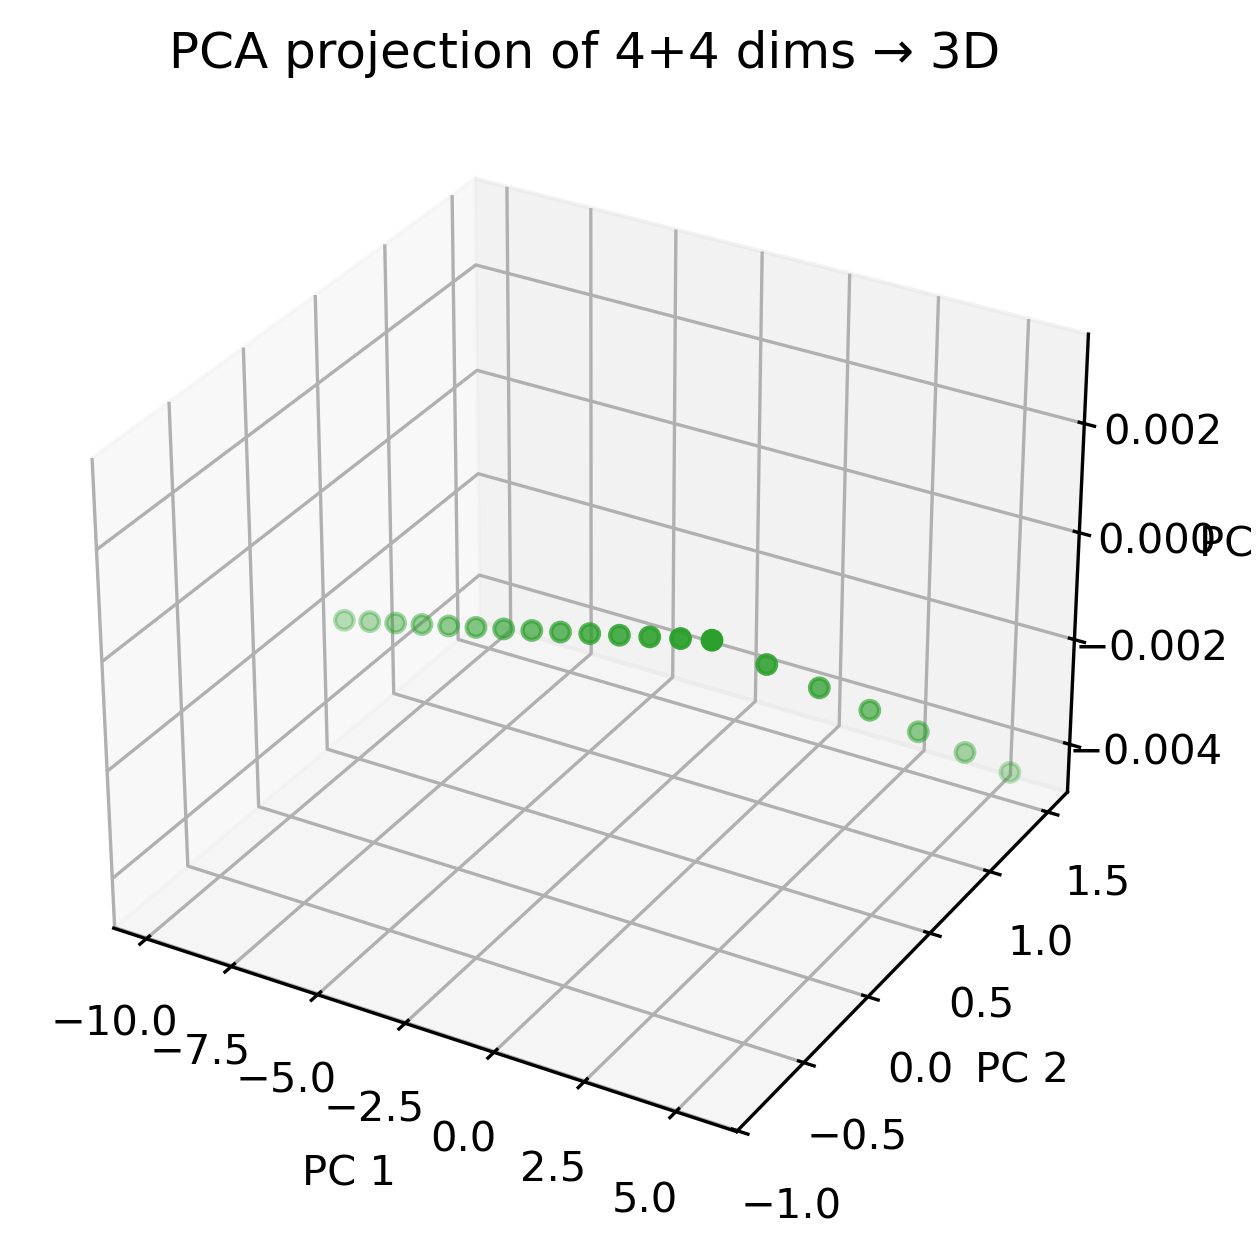
\includegraphics[width=\linewidth]{usage_target_optimized_degree_1.png}
    \end{minipage}\hfill
    \begin{minipage}{0.48\linewidth}
        \centering
        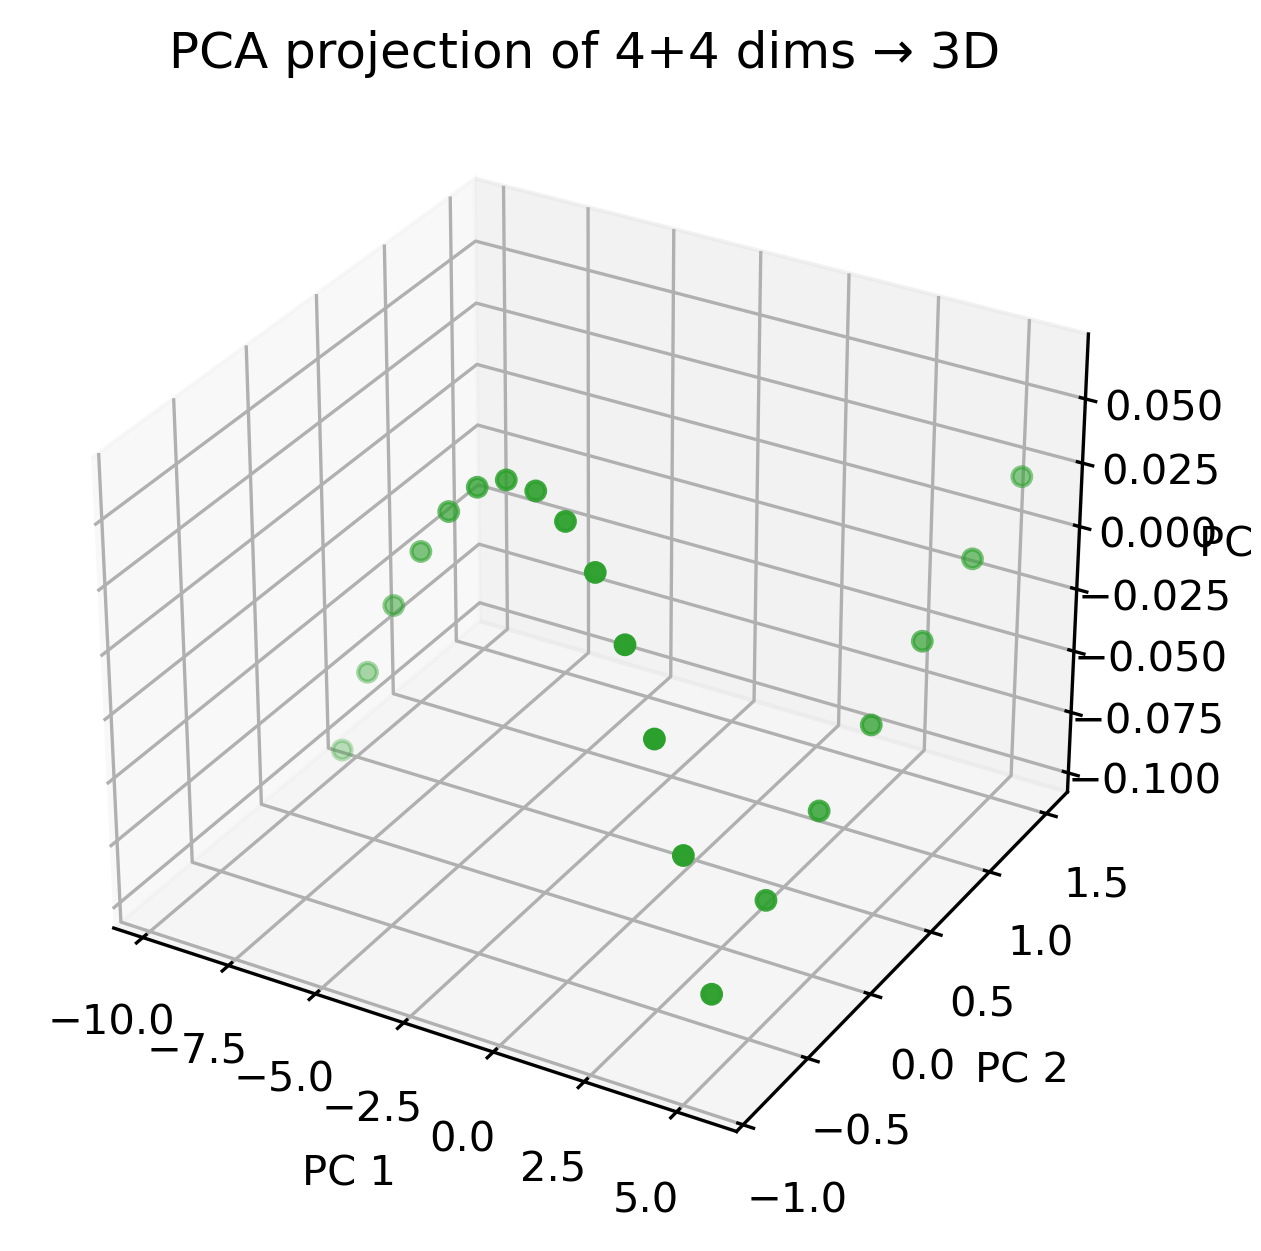
\includegraphics[width=\linewidth]{usage_target_optimized_degree_3.png}\\[0.5em]
        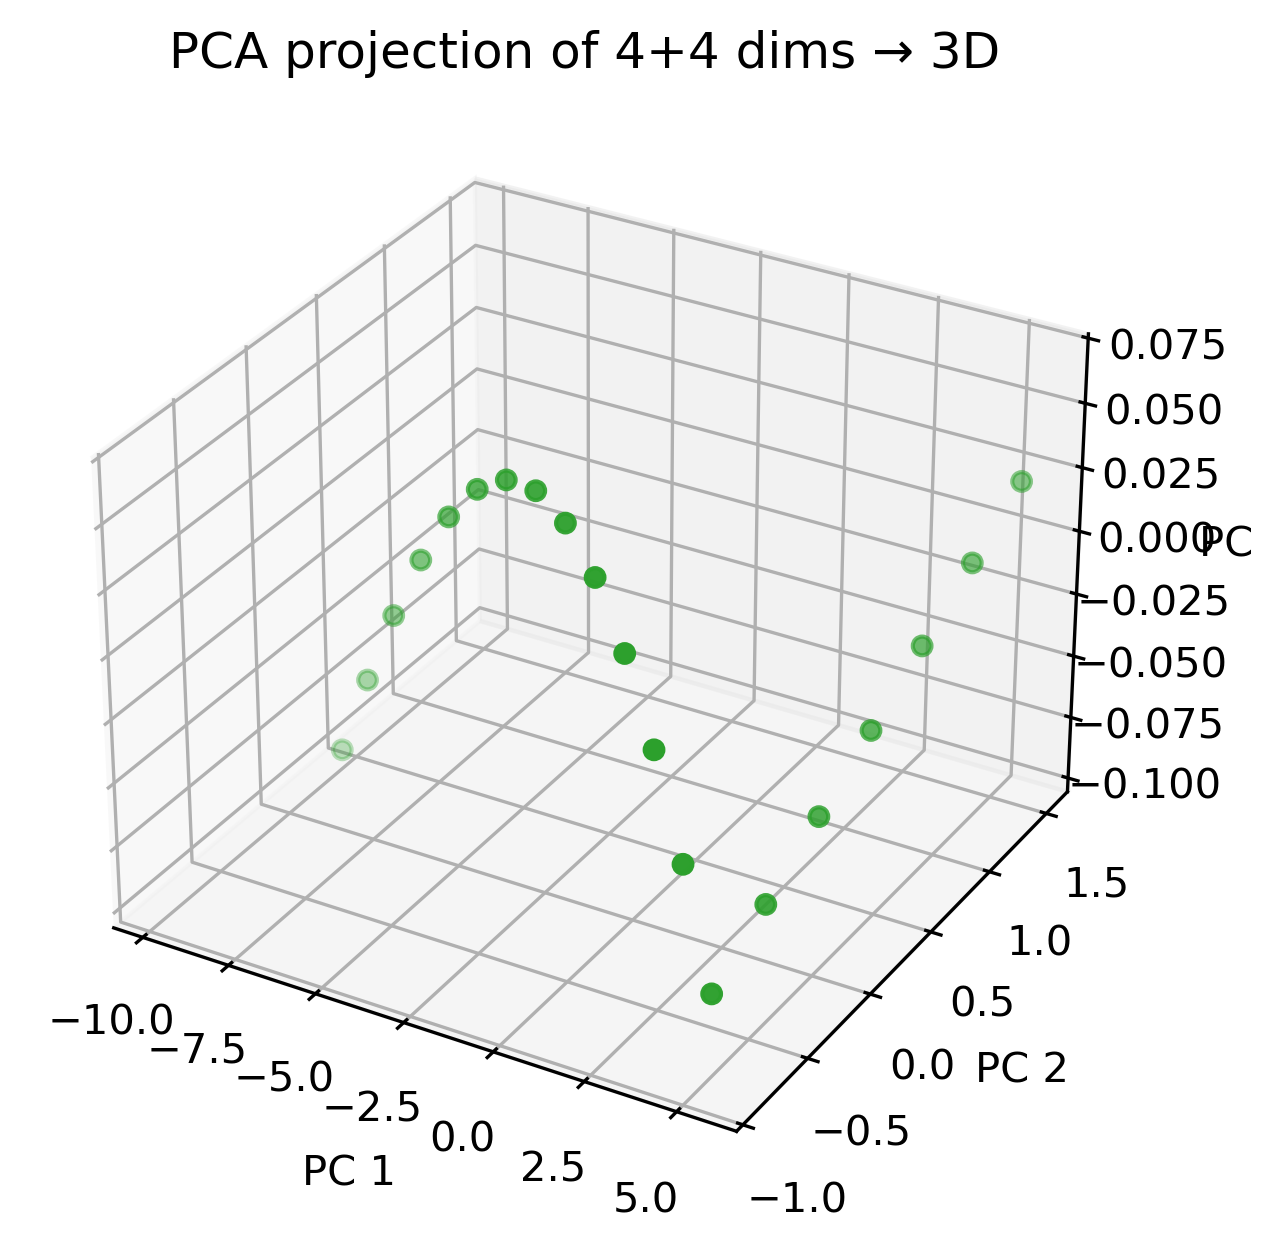
\includegraphics[width=\linewidth]{usage_target_optimized_degree_5.png}
    \end{minipage}
    \caption{Protótipo 4$\times$4: projeção PCA do conjunto (topo esquerdo)
    e reconstruções otimizadas para graus 1, 3 e 5 respectivamente no canto inferior esquerdo, superior direito e inferior direito.}
    \label{fig:target-dataset}
\end{figure}

\begin{figure}[H]
    \centering
    \begin{minipage}{0.48\linewidth}
        \centering
        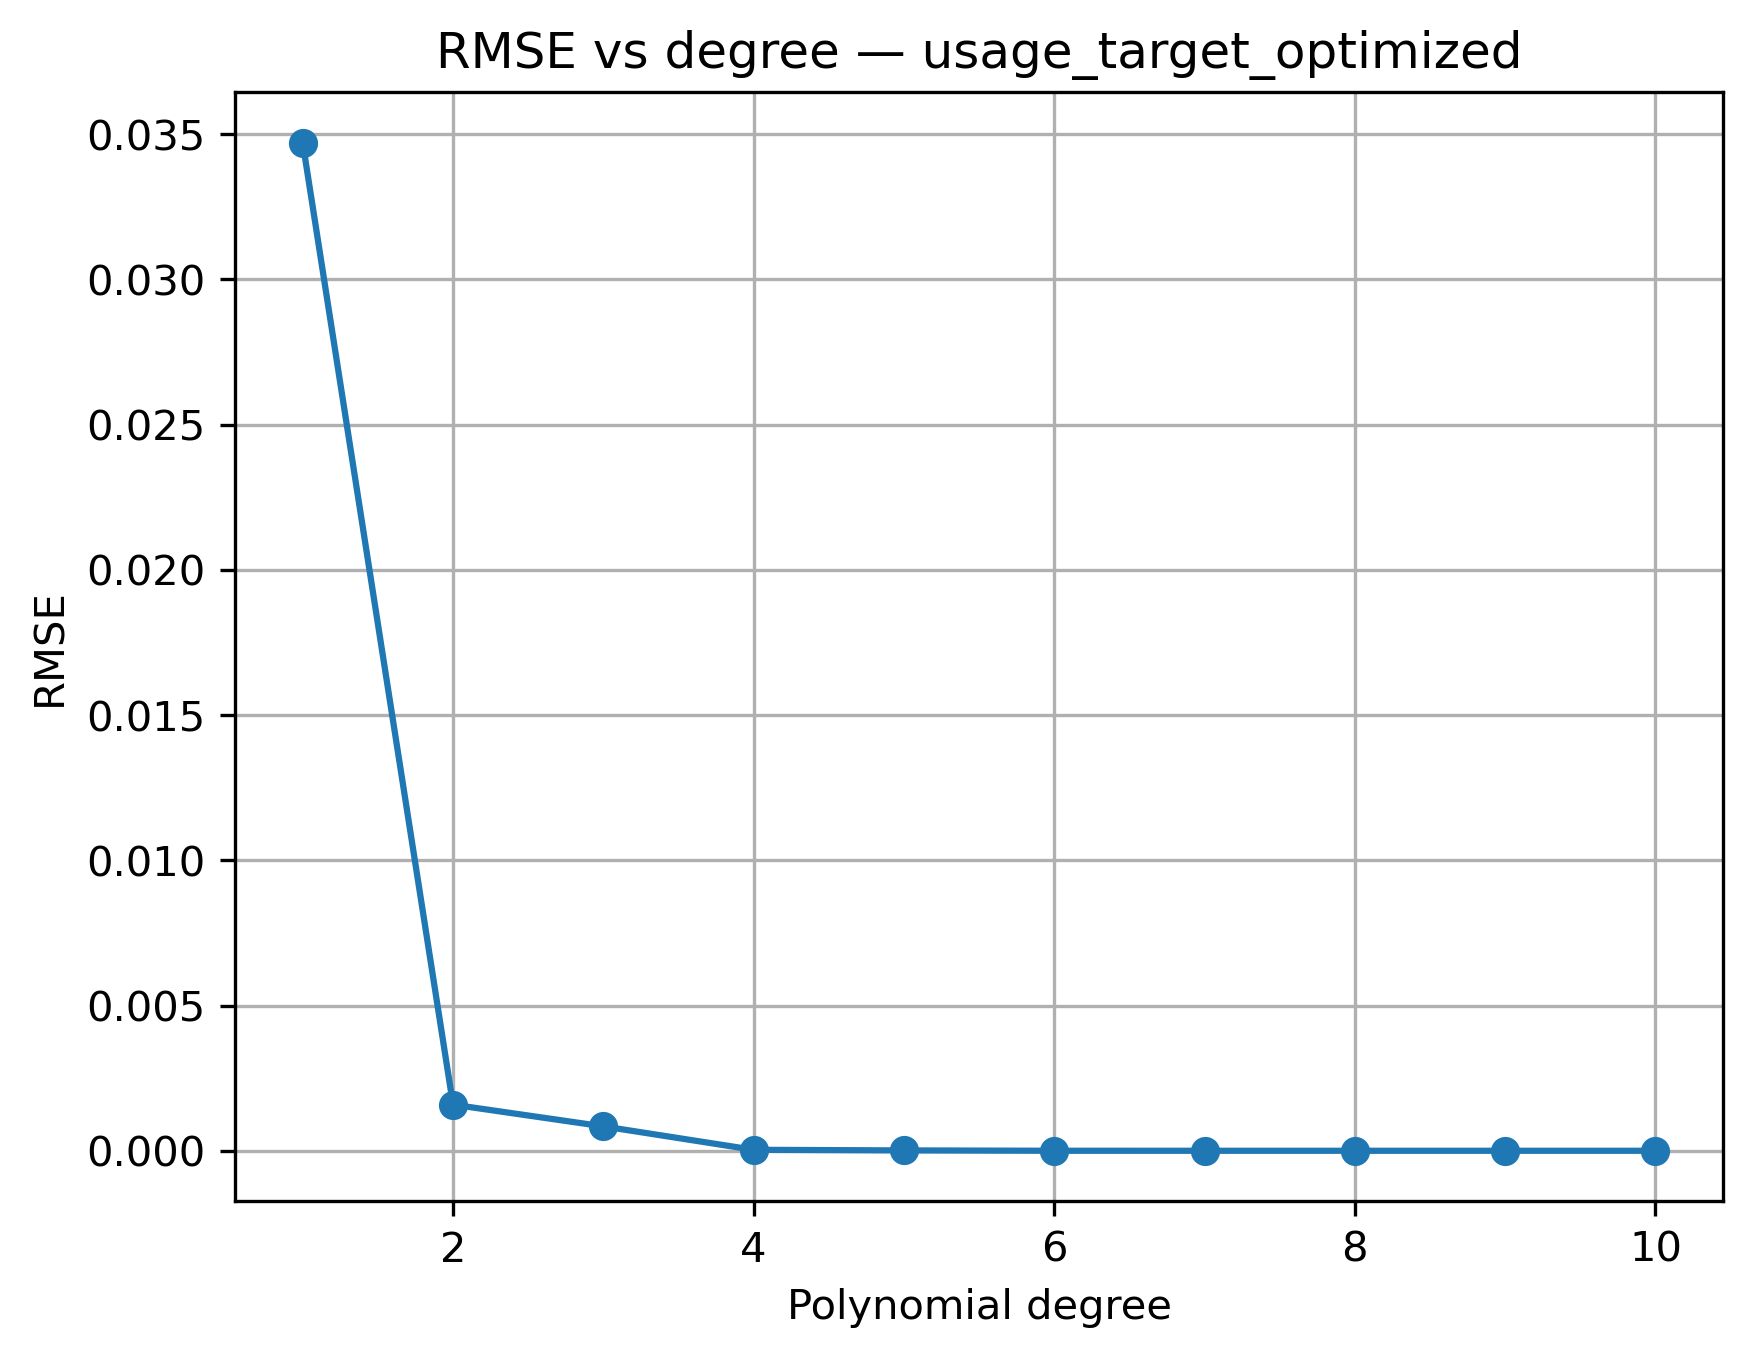
\includegraphics[width=\linewidth]{usage_target_optimized_rmse.png}
    \end{minipage}\hfill
    \begin{minipage}{0.48\linewidth}
        \centering
        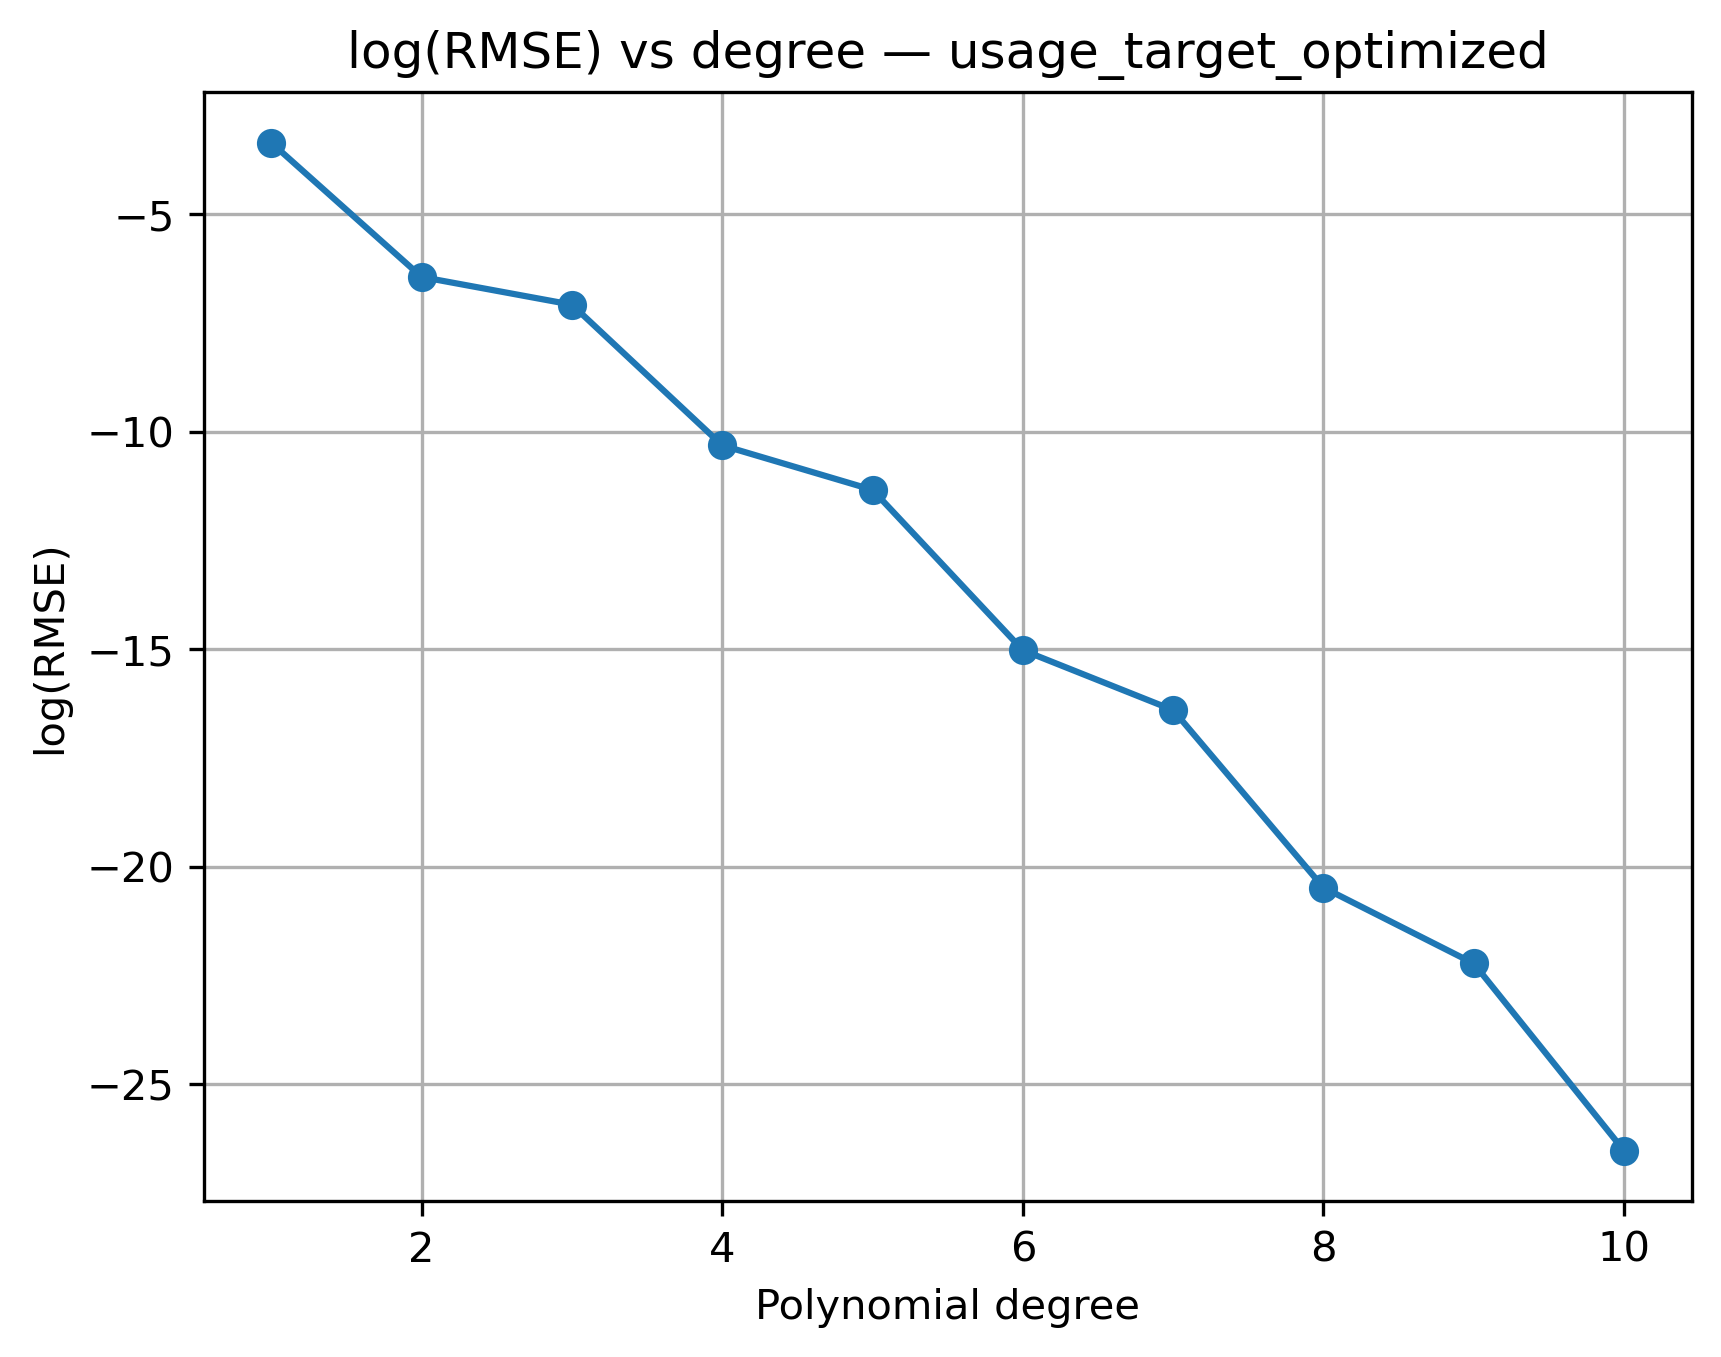
\includegraphics[width=\linewidth]{usage_target_optimized_rmse_log.png}
    \end{minipage}
    \caption{RMSE absoluto e logarítmico para o protótipo 4$\times$4.}
    \label{fig:target-metrics}
\end{figure}

\subsection{Problema extra: superfície da asa}

A superfície ``wing'' aplica nossa técnica em um estudo extra inspirado na aplicação
aeronáutica. A Figura~\ref{fig:wing-dataset} evidencia que o modelo de grau~7 se
ajusta à topologia da asa sem introduzir artefatos, mantendo resíduos entre
$-2{,}26$ e \num{1.98} com média praticamente nula e desvio padrão \num{0.613}.
O sweep de graus da Figura~\ref{fig:wing-metrics} mostra que termos de quarta
ordem já explicam \num[round-mode=places,round-precision=1]{\wingDegreeFourRtwoPercent}\%
da variância, enquanto o grau~7 alcança $R^2 = \num{\wingFullRtwo}$
(\num[round-mode=places,round-precision=1]{\wingFullRtwoPercent}\%) com RMSE de
\num{\wingFullRmse}. A combinação entre projeções PCA e contornos de resíduos
confirma que os erros restantes concentram-se nas bordas da superfície, regiões
com menor densidade de amostras, sugerindo o uso de ponderações futuras para
melhorar a extrapolação.

\begin{figure}[H]
    \centering
    \begin{minipage}{0.48\linewidth}
        \centering
        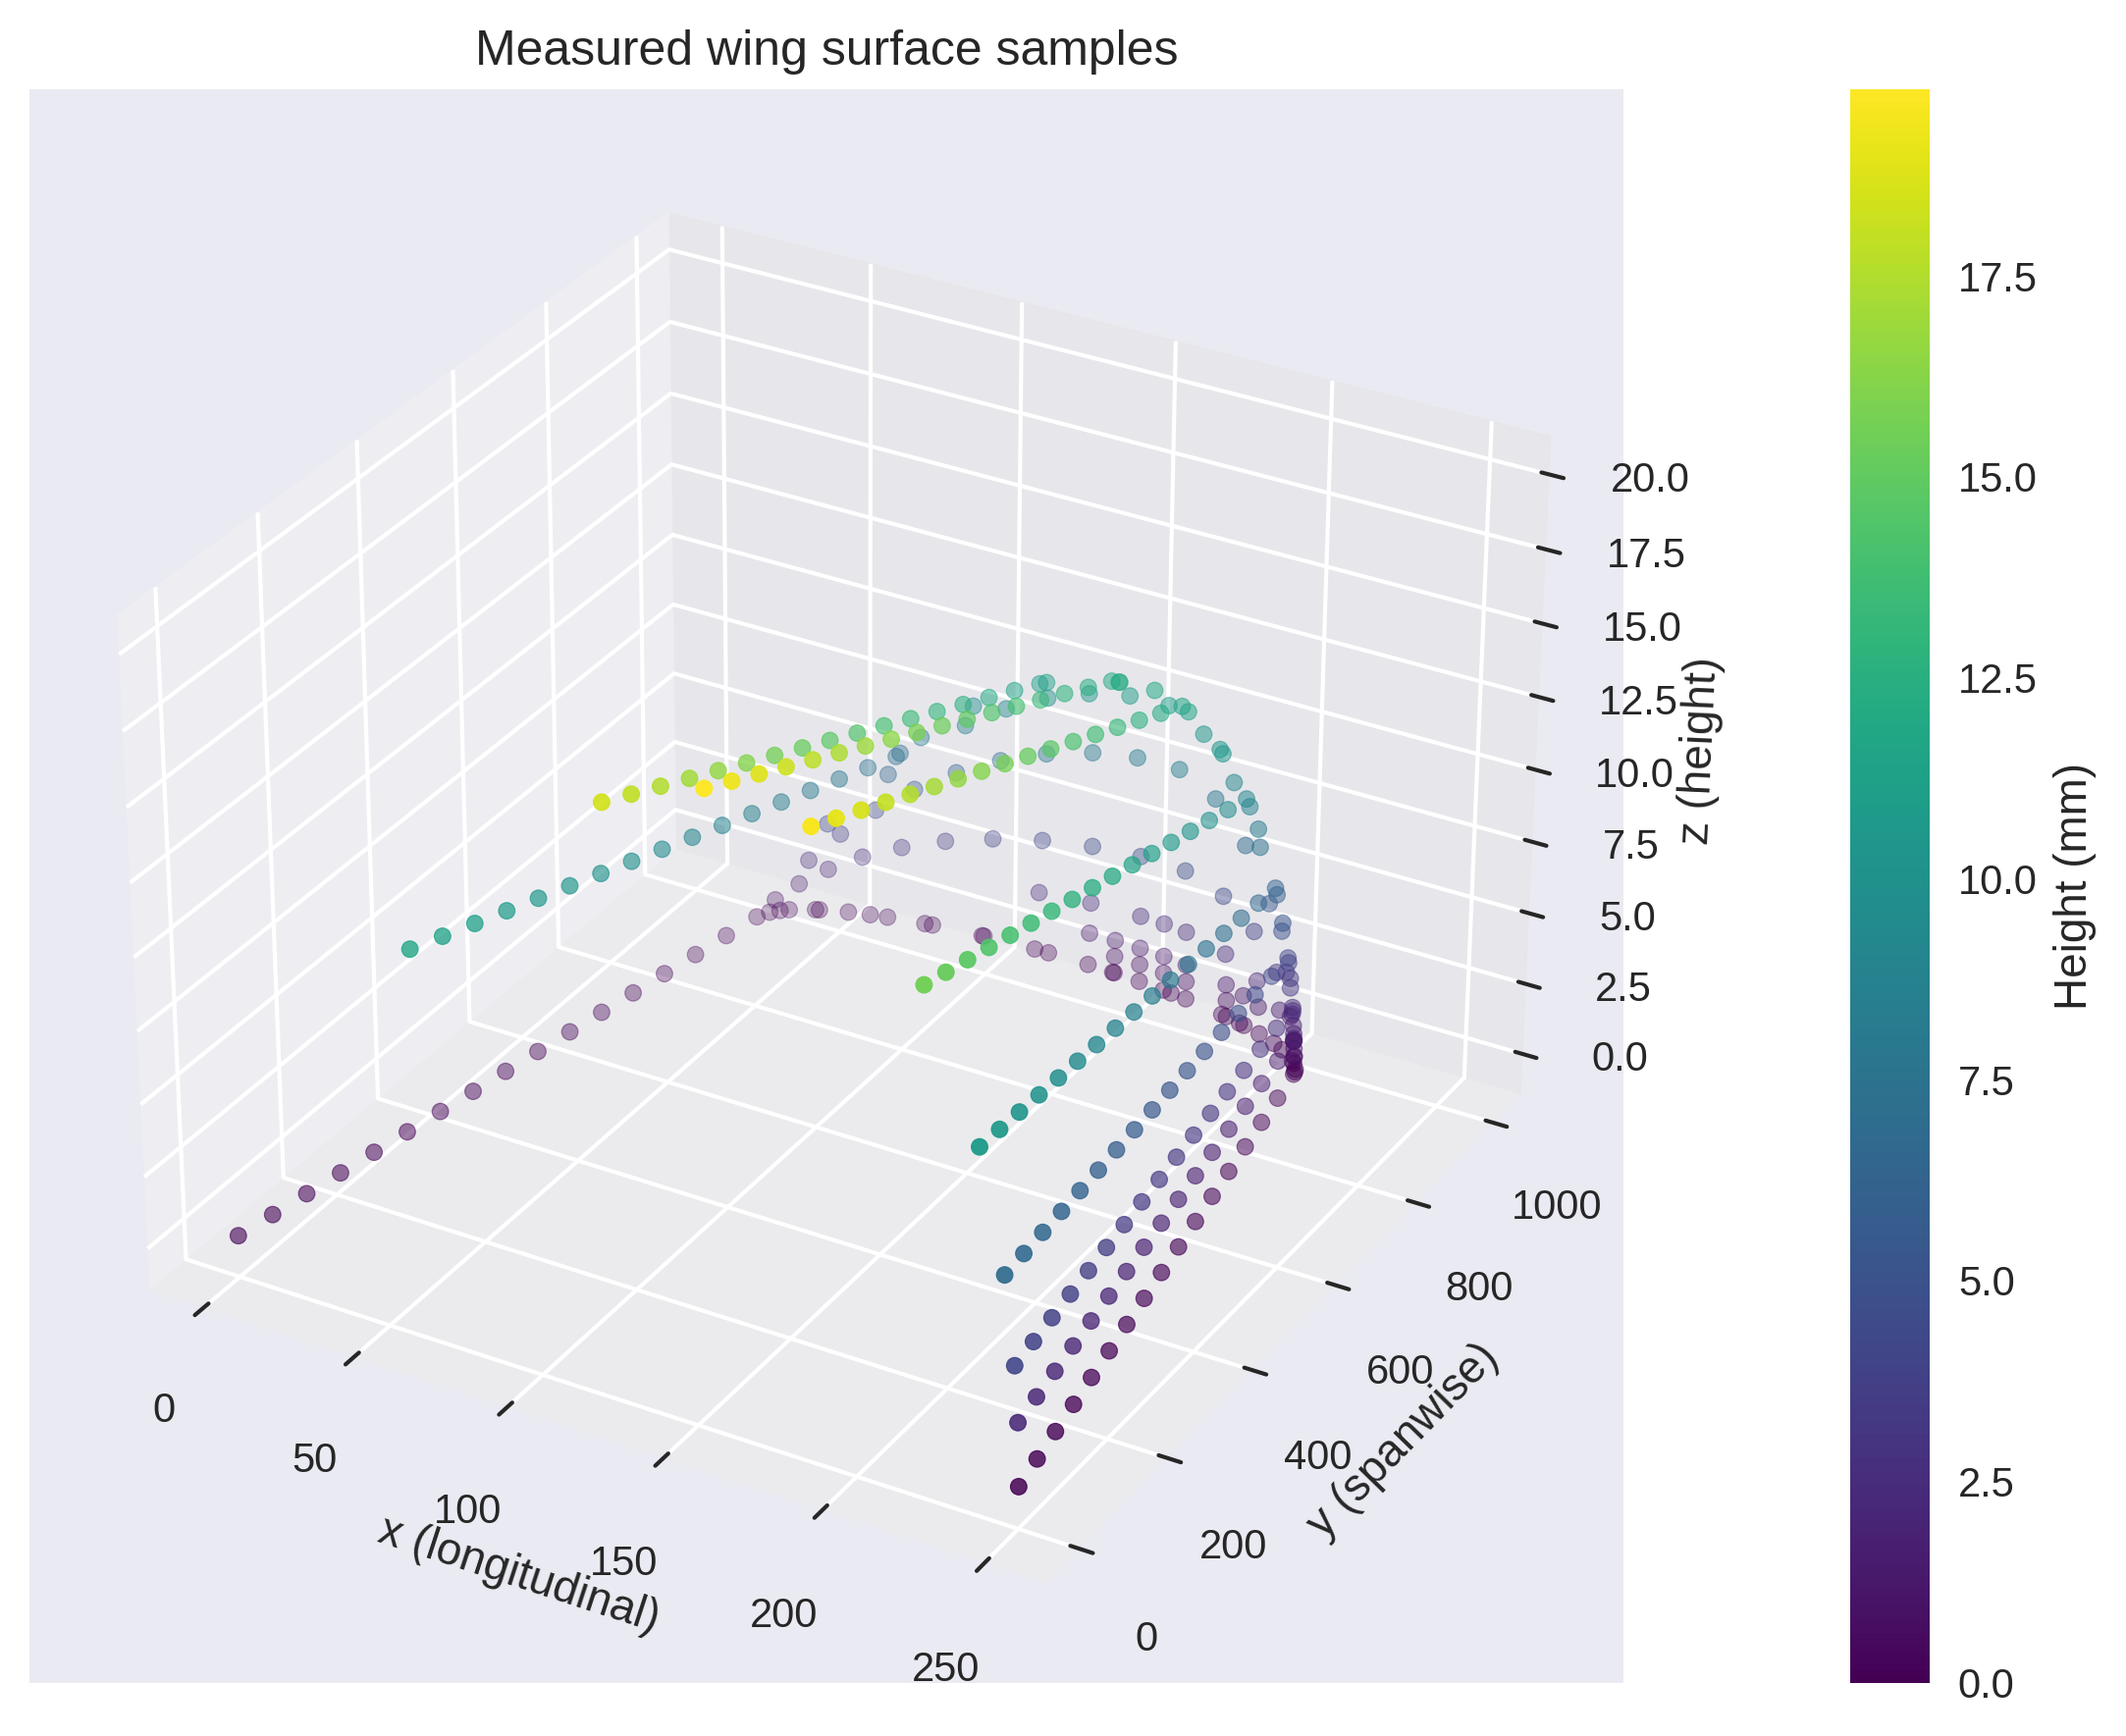
\includegraphics[width=\linewidth]{wing_samples_points.png}\\[0.5em]
        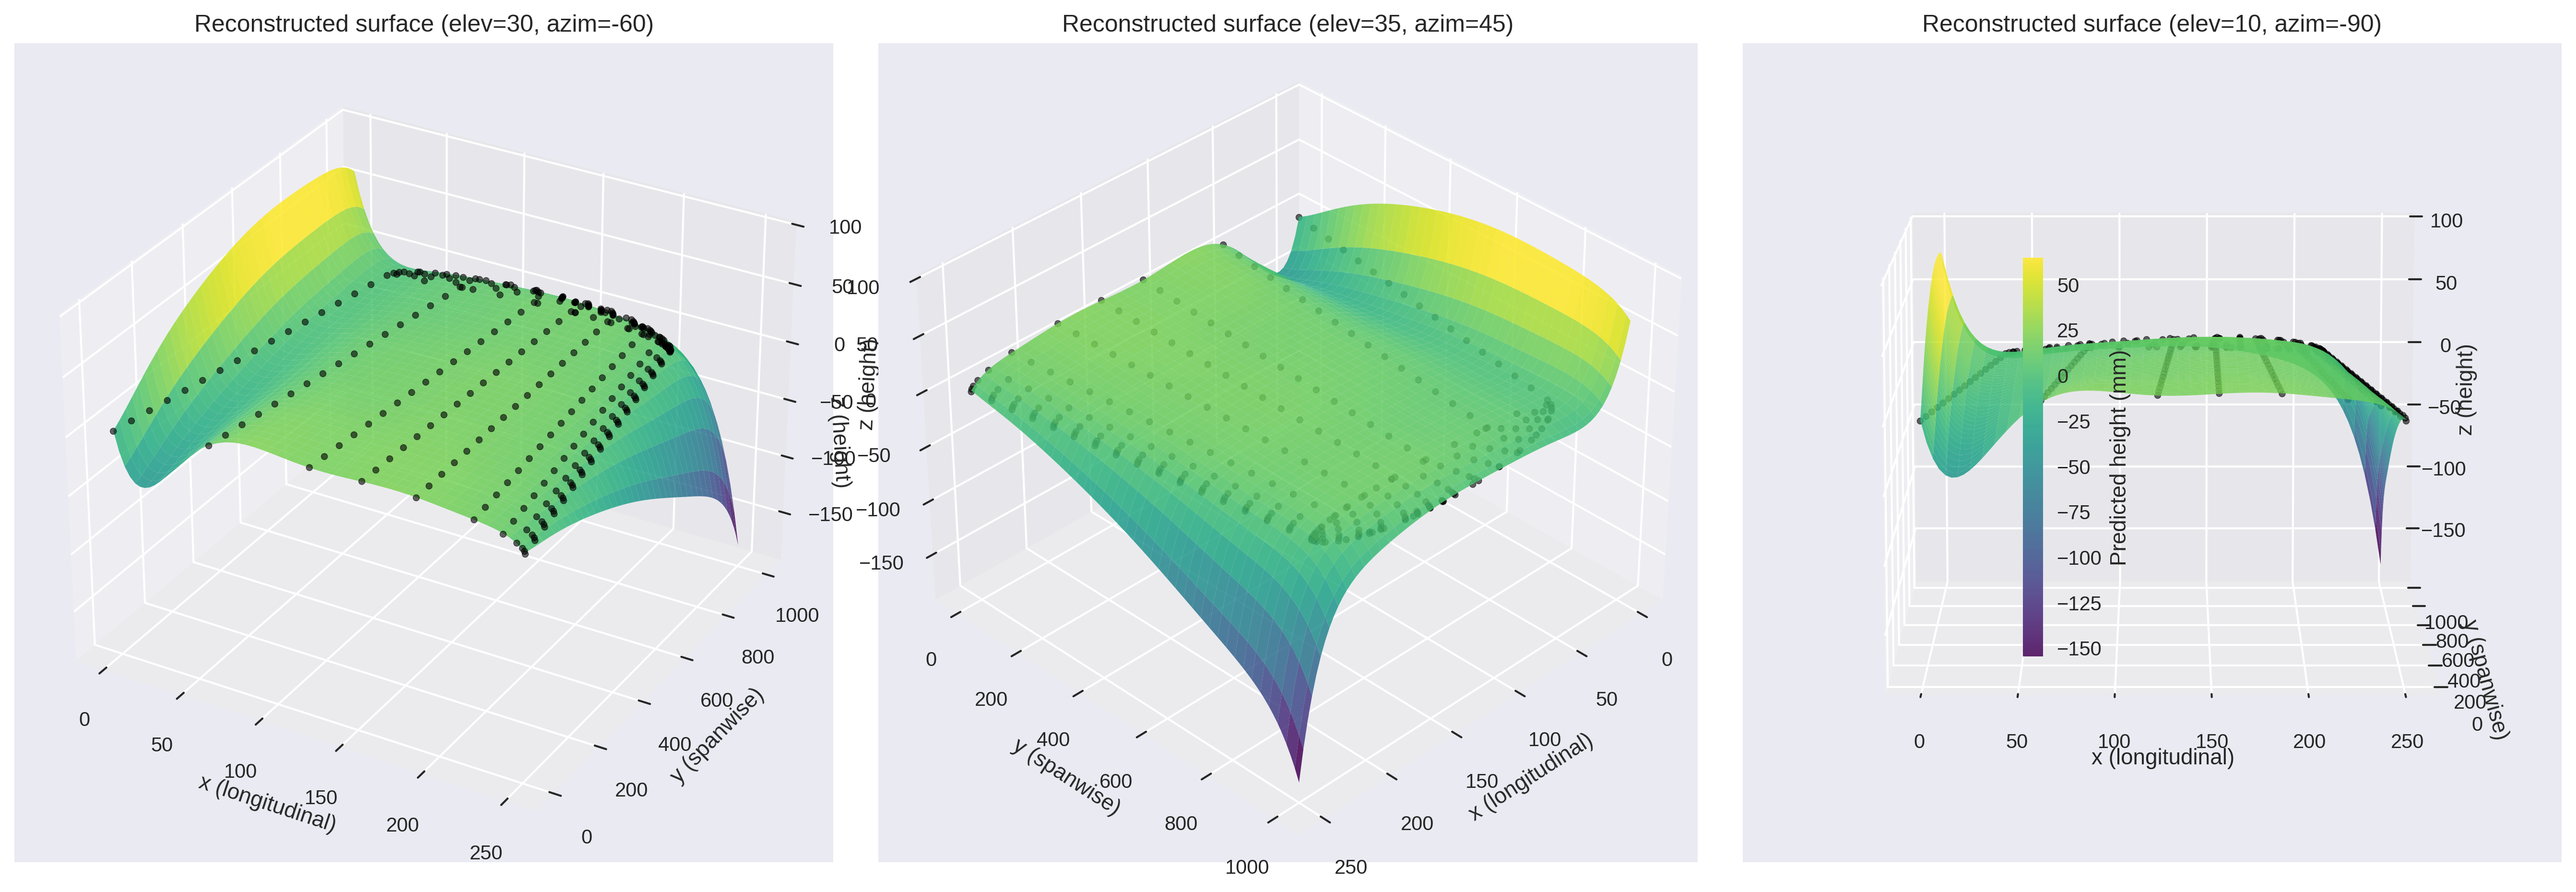
\includegraphics[width=\linewidth]{wing_surface_views.png}
    \end{minipage}\hfill
    \begin{minipage}{0.48\linewidth}
        \centering
        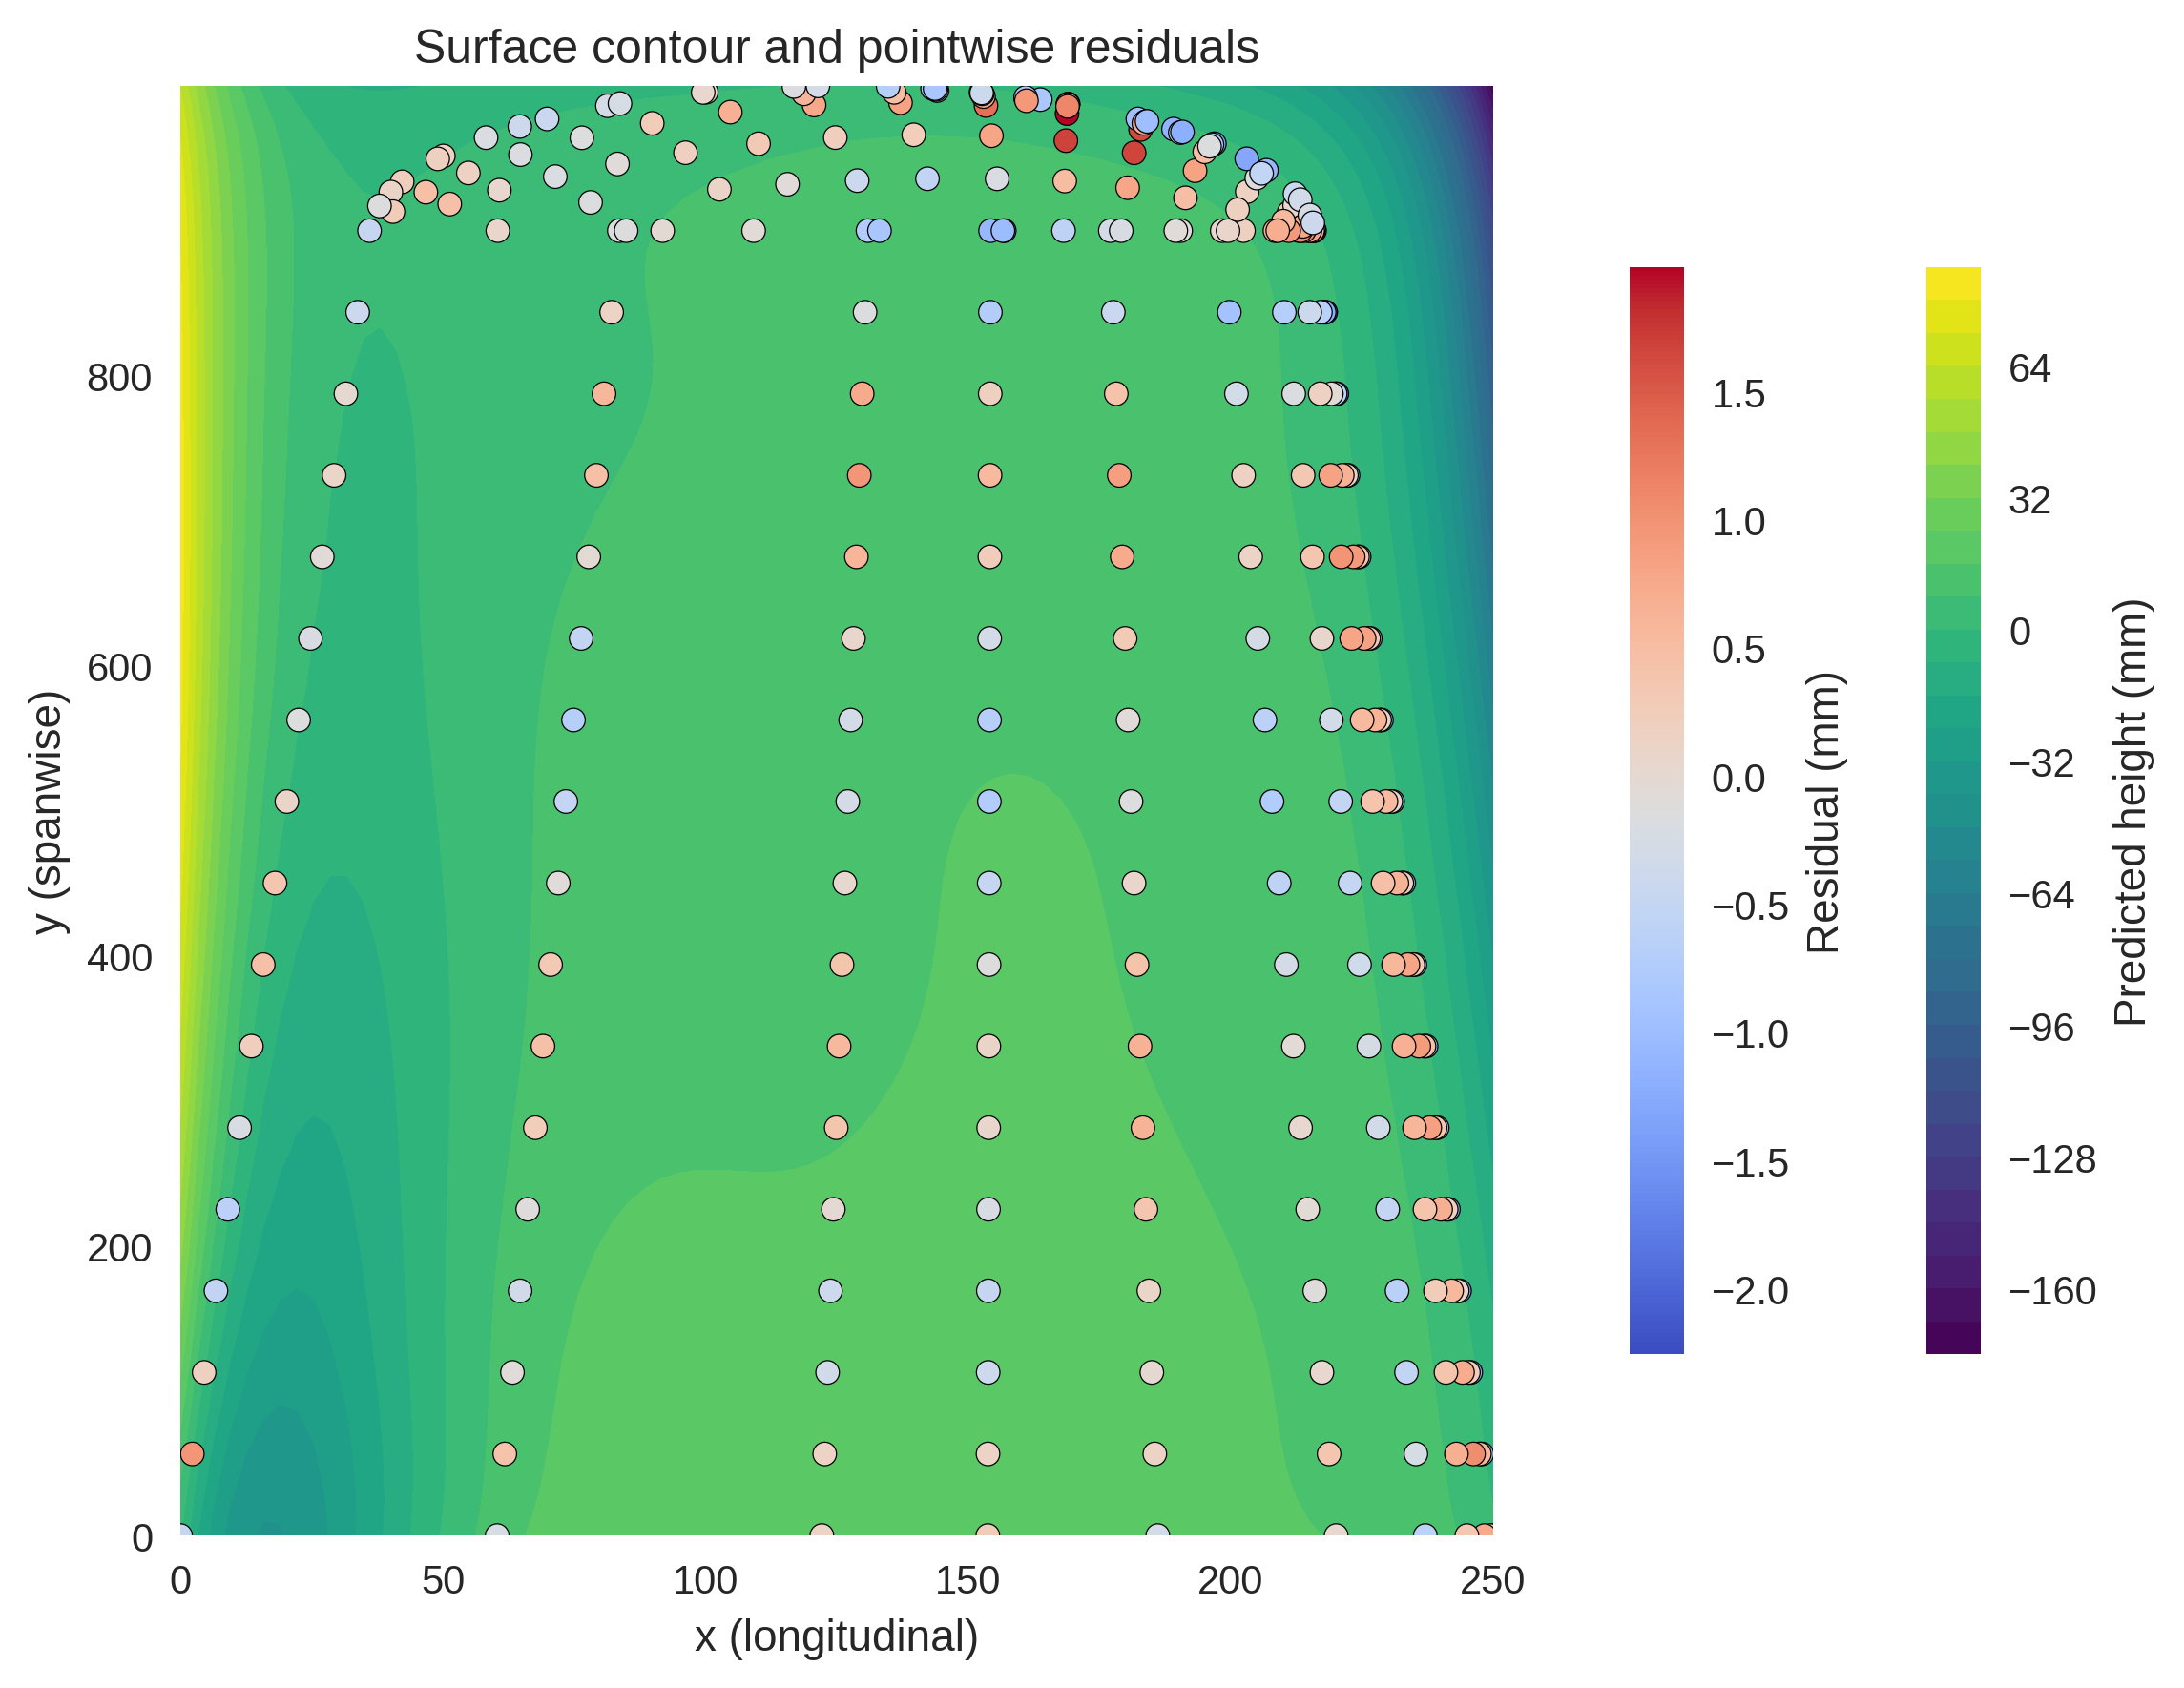
\includegraphics[width=\linewidth]{wing_contour_residuals.png}
    \end{minipage}
    \caption{Conjunto ``wing'': amostras, reconstruções e diagnóstico espacial
    dos resíduos.}
    \label{fig:wing-dataset}
\end{figure}

\begin{figure}[H]
    \centering
    \begin{minipage}{0.48\linewidth}
        \centering
        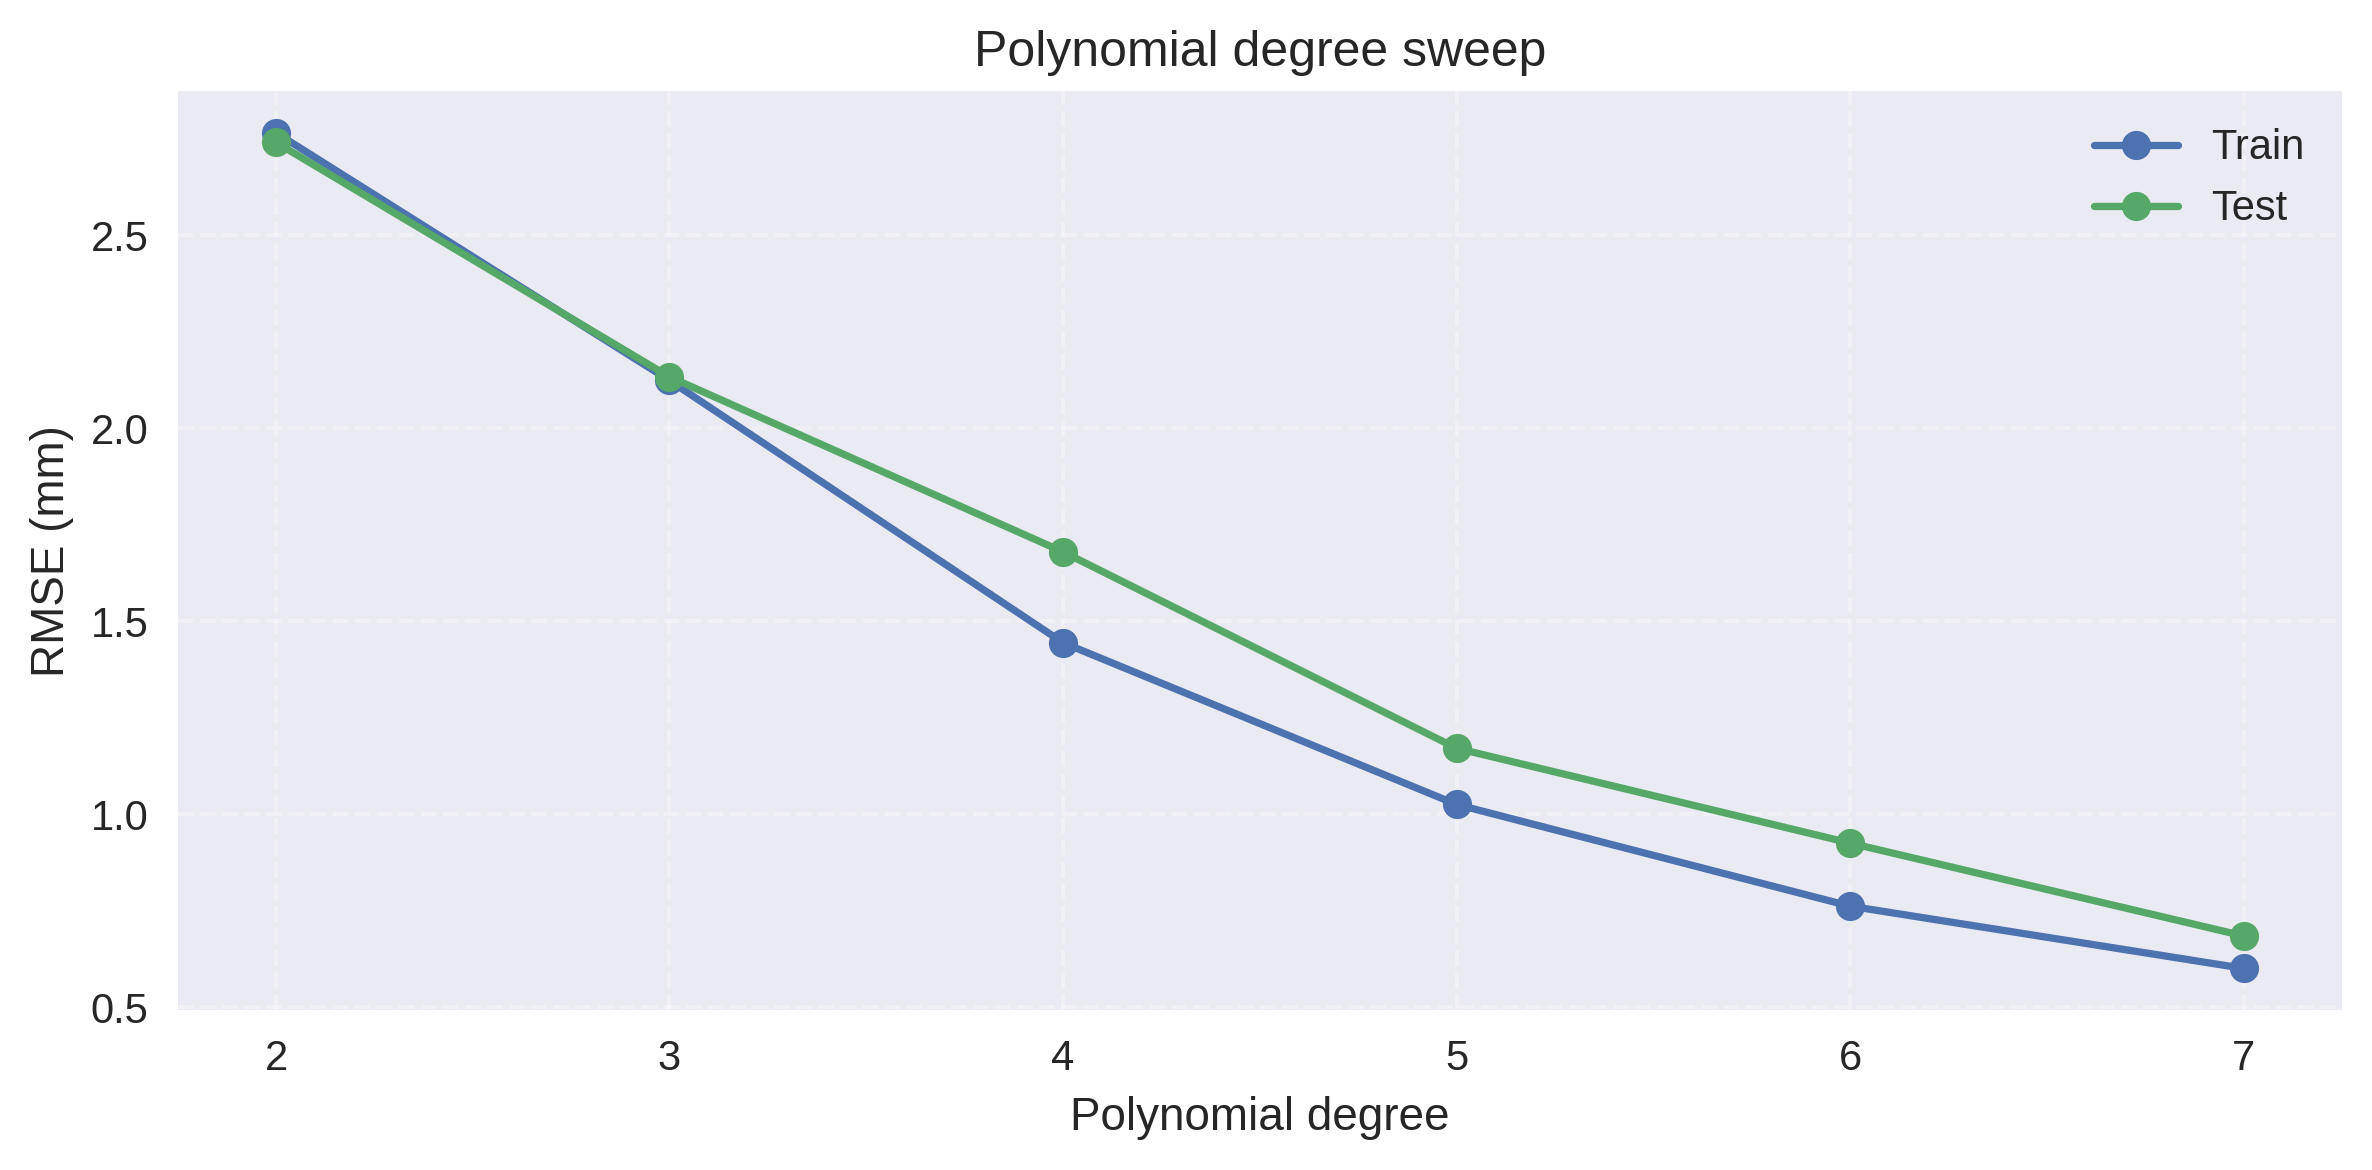
\includegraphics[width=\linewidth]{wing_degree_sweep.png}
    \end{minipage}\hfill
    \begin{minipage}{0.48\linewidth}
        \centering
        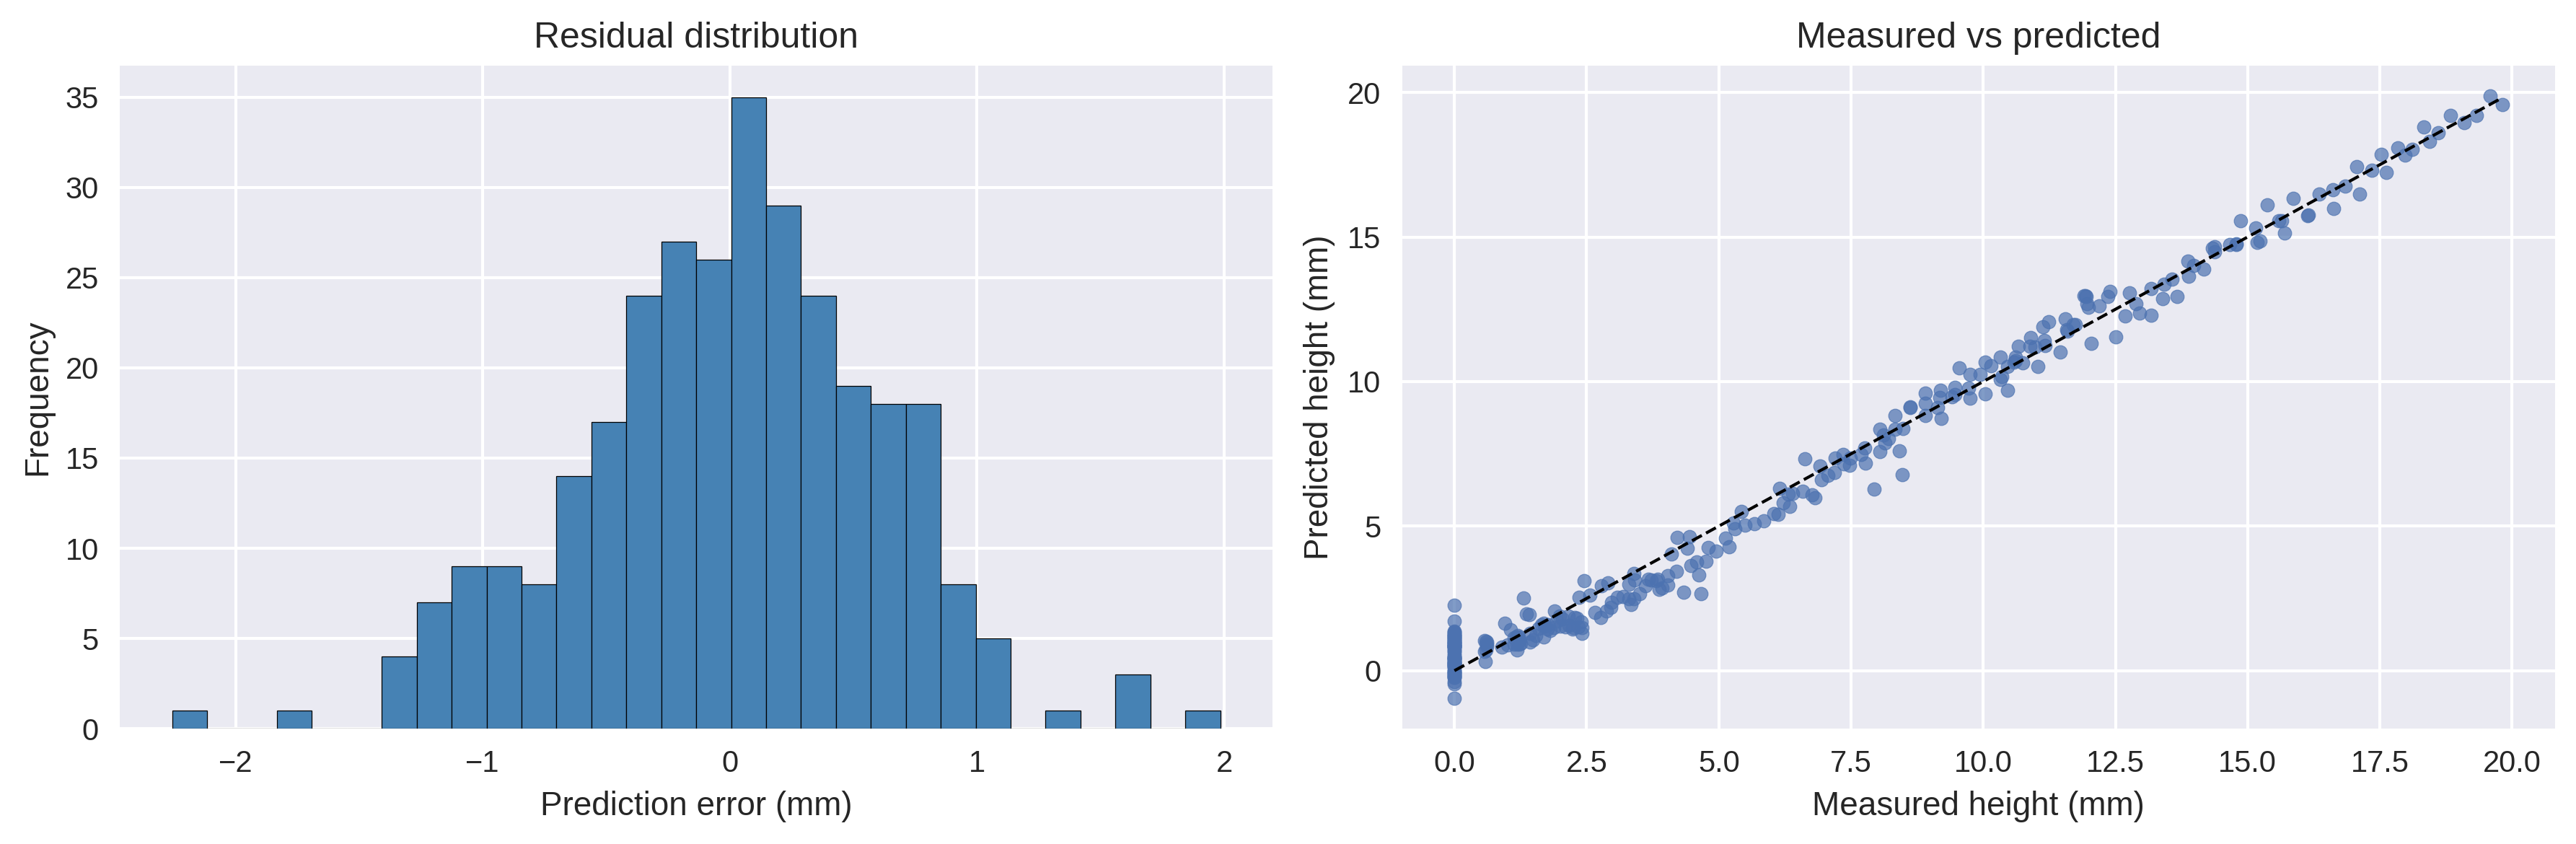
\includegraphics[width=\linewidth]{wing_residual_diagnostics.png}
    \end{minipage}
    \caption{Problema extra ``wing'': variação do erro com o grau (esquerda) e
    distribuição dos resíduos para grau~7 (direita).}
    \label{fig:wing-metrics}
\end{figure}



\subsection{Desempenho computacional}

Os ensaios de desempenho consolidam o impacto das otimizações introduzidas no
\texttt{regkit}. A Tabela~\ref{tab:benchmarks} resume os tempos médios de
execução e o pico de memória coletados para o caso didático com 200 pontos e
polinômios de grau cinco, bem como para o estresse com um milhão de pontos. A
transição da versão simbólica ingênua para o solver vetorizado reduz o tempo em
\num{\benchSpeedup} vezes e limita o uso de memória a apenas
\num[scientific-notation=false,round-mode=places,round-precision=1]{\benchMemPercent}\%
do valor original, sem alterar a acurácia. Já a extensão \textit{out-of-core}
preserva essencialmente o mesmo tempo do solver otimizado nessa escala, 
com custo computacional levemente maior, exibindo
variação relativa de
\num[scientific-notation=false,round-mode=places,round-precision=2]{\benchOocTimeVar}\%
no tempo e
\num[scientific-notation=false,round-mode=places,round-precision=2]{\benchOocMemVar}\%
no consumo de memória.

\begin{table}[H]
    \centering
    \caption{Tempo médio e pico de memória observados nos benchmarks.}
    \label{tab:benchmarks}
    \begin{tabular}{llcc}
        \hline\\
        Cenário & Implementação & Tempo [s] & Memória [MB]\\\\
        \hline\\
        200 pts, grau 5 & Naïve (symbolic) & \num{\benchNaiveTime} & \num{\benchNaiveMem}\\\\
                         & Optimized block solve & \num{\benchOptTime} & \num{\benchOptMem}\\\\
                         & Out-of-core largeP & \num{\benchOocTime} & \num{\benchOocMem}\\\\
        $10^{6}$ pts, grau 5 & Optimized block solve & \num{\benchHighOptTime} & \num{\benchHighOptMem}\\\\
                              & Out-of-core largeP & \num{\benchHighOocTime} & \num{\benchHighOocMem}\\\\
        \hline
    \end{tabular}
\end{table}

O caso de maior carga, ilustrado na Figura~\ref{fig:benchmark_high_load},
demonstra que o fluxo incremental realmente se diferencia quando a memória é o
recurso limitante: ao processar um milhão de pontos, o tempo cai cerca de
\num[scientific-notation=false,round-mode=places,round-precision=1]{\benchHighTimeDrop}\%
e o pico de memória despenca de
\num[scientific-notation=false,round-mode=places,round-precision=0]{\benchHighOptMem}~MB
para
\num[scientific-notation=false,round-mode=places,round-precision=2]{\benchHighOocMem}~MB.
Essa folga viabiliza regressões de alta resolução em estações com recursos
limitados e prepara o terreno para experimentos ainda mais extensos. 

A comparação entre as implementações confirma o objetivo do projeto: 
a versão ingênua serve apenas como referência didática, 
enquanto o solver otimizado é significativamente mais rápido e eficiente, 
sendo indicado para a maioria dos experimentos. 
Já a variante \textit{out-of-core}, 
embora apresente leve aumento no tempo de execução, 
permite o processamento de conjuntos de dados maiores e é recomendada para cenários com restrições de memória.


\begin{figure}[H]
    \centering
    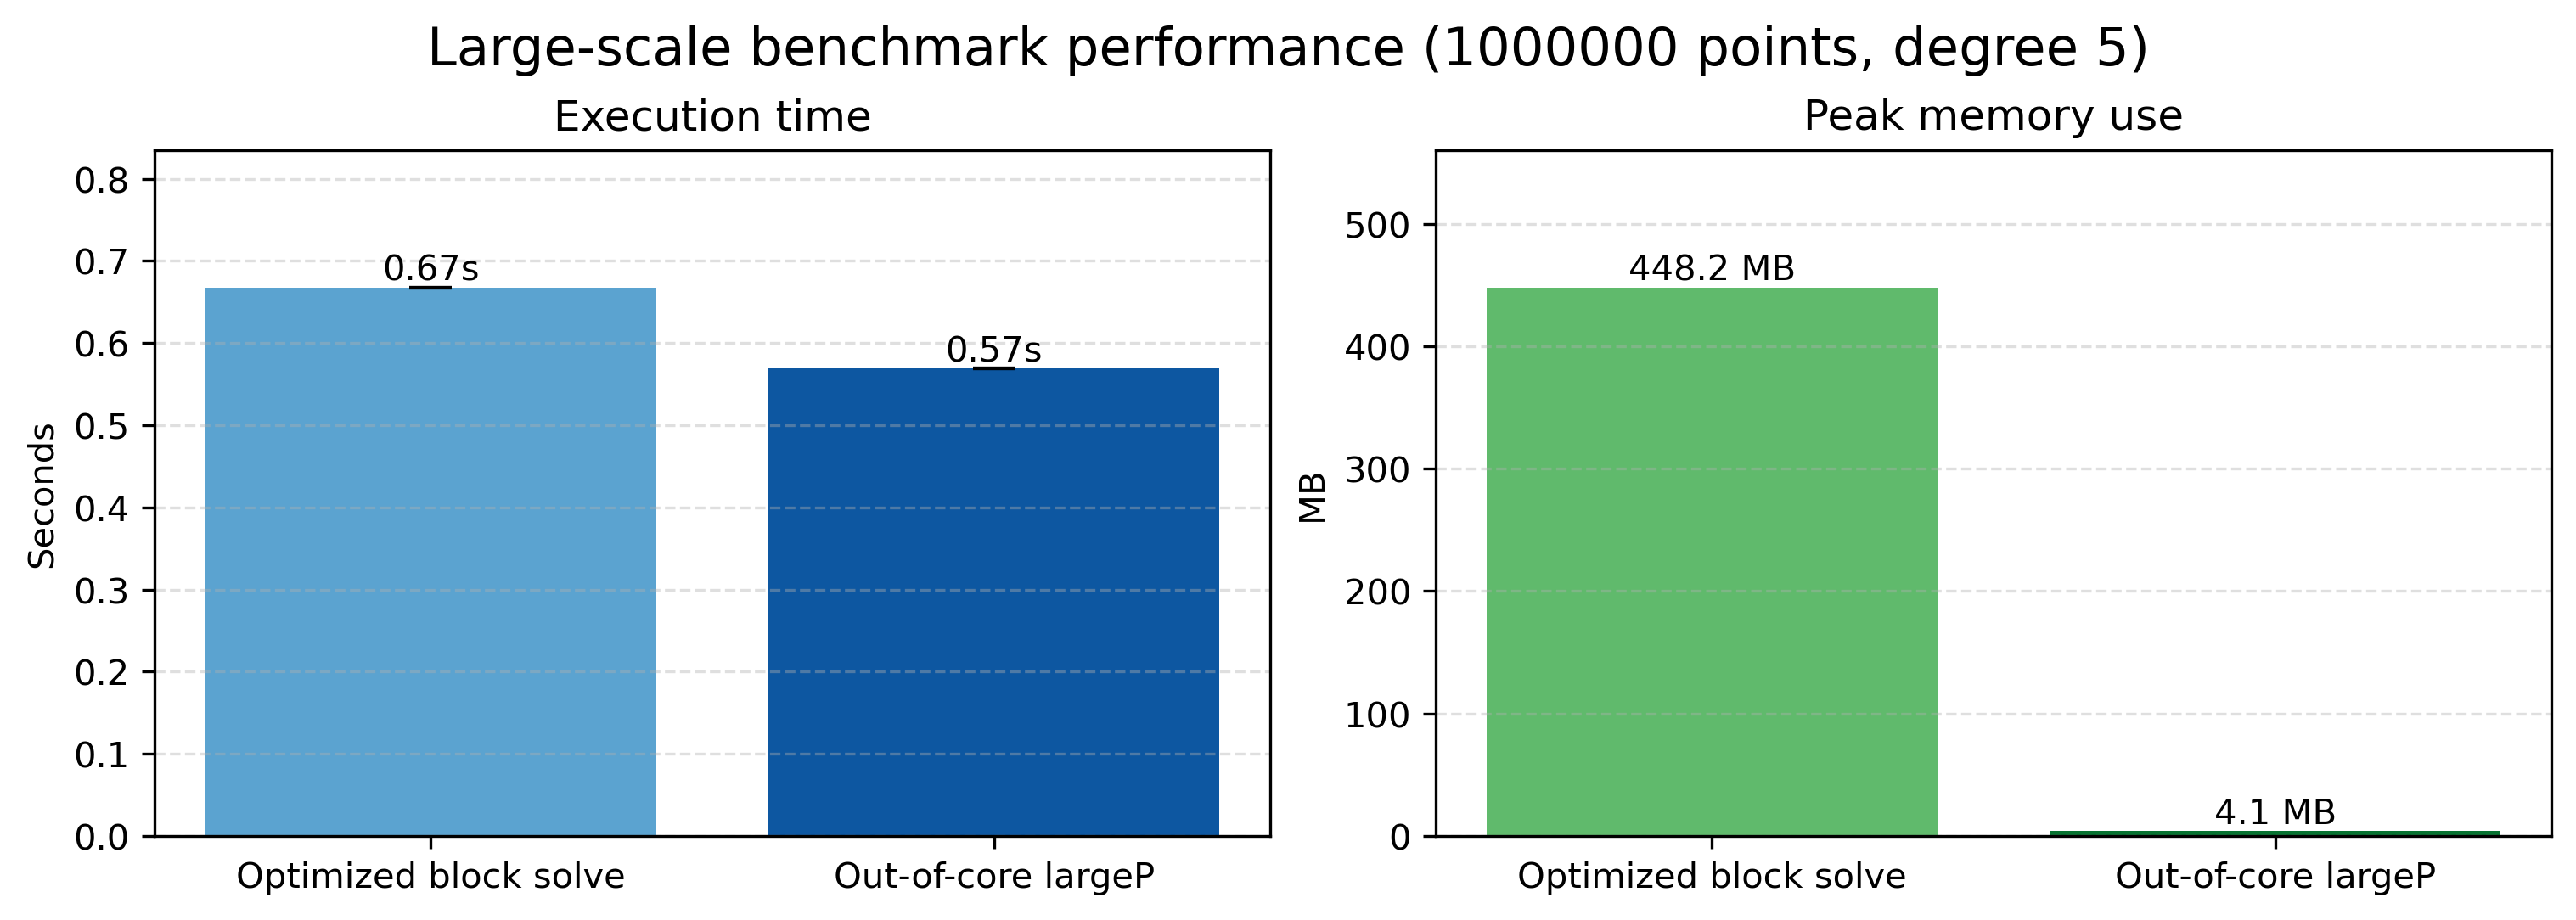
\includegraphics[width=0.9\linewidth]{benchmark_high_load_bars.png}
    \caption{Tempo e memória medidos no estresse com um milhão de pontos.}
    \label{fig:benchmark_high_load}
\end{figure}

\subsection{Condicionamento Numérico}

\pgfplotstableread[col sep=comma]{../../results/ill_conditioned_gram.csv}\illconditioned

\pgfplotstablegetelem{0}{num_points}\of\illconditioned
\edef\illHighPoints{\pgfplotsretval}
\pgfplotstablegetelem{0}{degree}\of\illconditioned
\edef\illHighDegree{\pgfplotsretval}
\pgfplotstablegetelem{0}{cond}\of\illconditioned
\edef\illHighCondRaw{\pgfplotsretval}
\pgfplotstablegetelem{1}{ridge_effective}\of\illconditioned
\edef\illHighRidge{\pgfplotsretval}

\pgfplotstablegetelem{2}{num_points}\of\illconditioned
\edef\illDupPoints{\pgfplotsretval}
\pgfplotstablegetelem{2}{degree}\of\illconditioned
\edef\illDupDegree{\pgfplotsretval}
\pgfplotstablegetelem{2}{cond}\of\illconditioned
\edef\illDupCondRaw{\pgfplotsretval}

\edef\illHighCond{\fpeval{\illHighCondRaw}}

Experimentos controlados confirmaram que certas configurações tornam o bloco de
Gram extremamente mal condicionado.
Um script dedicado\footnote{Disponível no repositório como
\texttt{experiments/run\_ill\_conditioned\_regression.py}, o qual gera a
tabela \texttt{results/ill\_conditioned\_gram.csv}.}
reproduz dois cenários representativos: (i)
\illHighPoints\,amostras equiespaçadas em $[-1,1]$ ajustadas com um polinômio
de grau \illHighDegree, cuja matriz apresenta
$\operatorname{cond}(G) \approx
\num[scientific-notation=true,round-mode=figures,round-precision=3]{\illHighCond}$;
e (ii) \illDupPoints\,amostras coincidentes sob ajuste de grau
\illDupDegree, para as quais $\operatorname{cond}(G)$ é reportado como
\texttt{\illDupCondRaw}, evidenciando a degenerescência da matriz de
Vandermonde.

Denotemos por $V \in \mathbb{R}^{N \times p}$ a matriz de
Vandermonde cujas linhas são os vetores de monômios avaliados em cada ponto
$p_j$ e cujas colunas correspondem às $p=\binom{n+r}{r}$ funções base.
Ao acumular $V^T V$ ao longo das amostras, obtemos precisamente o bloco de
Gram $G$, enquanto a acumulação $V^T \vec{f}$ gera o vetor $\vec{b}$.
Quando as colunas de $V$ ficam quase linearmente dependentes - como ocorre em
graus altos, em domínios muito alongados ou em variáveis fortemente
correlacionadas - essa acumulação herda a perda de significância e culmina em
um $G$ mal condicionado.

Para mitigar tais problemas, o solver \texttt{regression\_optimized} foi projetado para identificar automaticamente situações de mal condicionamento e, nesses casos,
ele substitui a resolução em blocos por uma chamada a
\texttt{numpy.linalg.lstsq}, enquanto \texttt{regression\_largeP} mantém a
decomposição, porém injeta automaticamente uma regularização de magnitude
\num[scientific-notation=true]{\illHighRidge} no sistema, conforme registrado
para ambos os cenários analisados.

